\chapter{Resultados Numéricos}\label{ch:results}

En este capítulo presentaremos varios experimentos numéricos y
comprobaremos que los resultados concuerdan con la teoría estudiada
en los capítulos anteriores.
Introduciremos las condiciones iniciales que posteriormente serán
empleadas para implementar estos experimentos numéricos, resueltos
mediante simulaciones numéricas con el ordenador.
Para ello, haremos uso del lenguaje de programación
Python\footnote{\url{Disponible en https://carlosal1015.github.io/finite-volume-hyperbolic-problems/notebook}}.

\section{Condiciones de contorno}

Las condiciones de contorno deben especificarse de forma adecuada
para que un problema formulado en términos de EDP esté bien planteado.
Como norma general, el saber cuál es la estructura de las rectas
características, nos proporciona cuantas condiciones de contorno se
necesitan en función del método numérico empleado.
Un enfoque sería extender el dominio computacional para incluir
celdas adicionales en cada extremo, denominadas celdas fantasmas,
cuyos valores se establecen al comienzo de cada paso de tiempo y que
en general dependen de los datos sobre la frotera y de las soluciones
interiores.
En esta memoria, se van a estudiar solamente esquemas numéricos de un
paso.
Por ello, no será necesario más de una celda fantasma en cada extremo.

Supongamos que $\left[a,b\right]$ es el dominio computacional del
problema, subdividido en las celdas $c_{1},c_{2},\dotsc,c_{N}$ donde
$c_{i}=\left(x_{i-\frac{1}{2}},x_{i+\frac{1}{2}}\right)$, para
$i=1,\dotsc,N$.
La figura 5.1 muestra una malla con una celda fantasma en cada
extremo.

En principio, usaremos condiciones de contorno periódicas, esto es,
para cada instante de tiempo $t_{n}$, impondremos la condición
$u^{n}_{0}=u^{n}_{N}$ si las rectas características tienen pendiente
positiva o la condición $u^{n}_{N+1}=u^{n}_{1}$, en caso contrario.

Además, usaremos condiciones de contorno Neumann homogéneas, donde
impondremos que la derivada direccional de la función $u$, variable
conservativa, en la dirección del vector normal unitario $n$, tal y
como fue definida en (2.26), sea conocida, por ejemplo igual a cero.
Luego, esta condición de contorno viene dada por

\begin{equation*}
    \diffp{u}{n}=
    n\cdot Du=
    0,\text{ para todo }x\in\partial\Omega,
\end{equation*}

donde $\partial\Omega$ es la frontera del dominio espacial.

\section{Primeros tests}

En esta sección vamos a realizar experimentos que ratifican algunos
resultados vistos en la teoría.
Estos experimentos van a ser aplicados a la ecuación de transporte
dada por

\begin{equation*}
    u_{t}
    \left(x,t\right)+
    cu_{x}
    \left(x,t\right)=
    0,\quad
    x\in\mathbb{R},\quad
    t>0,
\end{equation*}

siendo $c$ es la velocidad de propagación.
En el primer ejemplo, nos centraremos en el problema de Cauchy cuya
condición inicial viene dada por la ecuación (2.7), para un dato
inicial no regular (infinitamente derivable).
En el segundo ejemplo, nos centraremos en el problema de Riemann cuya
condición inicial viene dada por la ecuación (2.13), ambos problemas
estudiados en el capítulo 2.
Además, a partir de estas condiciones iniciales, obtenemos la
solución exacta en cualquier instante de tiempo posterior, dada por
la expresión (2.10) para el problema de Cauchy genérico y por la
expresión (2.14) para el problema de Riemann.
Entonces, comparamos en cada instante de tiempo la solución exacta
con la solución aproximada obtenida para cada uno de los esquemas
numéricos estudiados en el capítulo 4.

\subsection*{Ejemplo $1$}

En este ejemplo consideramos el dominio espacial
$\Omega=\left[0,20\right]$, el paso en espacio $\Delta x=0.1$, el
paso en tiempo $\Delta t=0.02$, la velocidad de propagación negativa
$c=-1$ (para los que se verifica la condición CFL) y la condición
inicial dada por

\begin{equation*}
    u_{0}=
    e^{-{\left(x-15\right)}^{2}}.
\end{equation*}

Para estos datos calculamos las soluciones numéricas de la ecuación
de transporte (5.1) con condición inicial, aplicando el método
descentrado downwind, el método de Lax-Friedrichs y por último, el
método de Lax-Wendroff.
Para ello, hemos empleado el lenguaje de programación Python.
Así, obtenemos los resultados de las figuras 5.2 y 5.3, para cada uno
de los métodos estudiados junto con la solución exacta para cada
instante de tiempo considerado.

\begin{figure}[ht!]
    \centering
    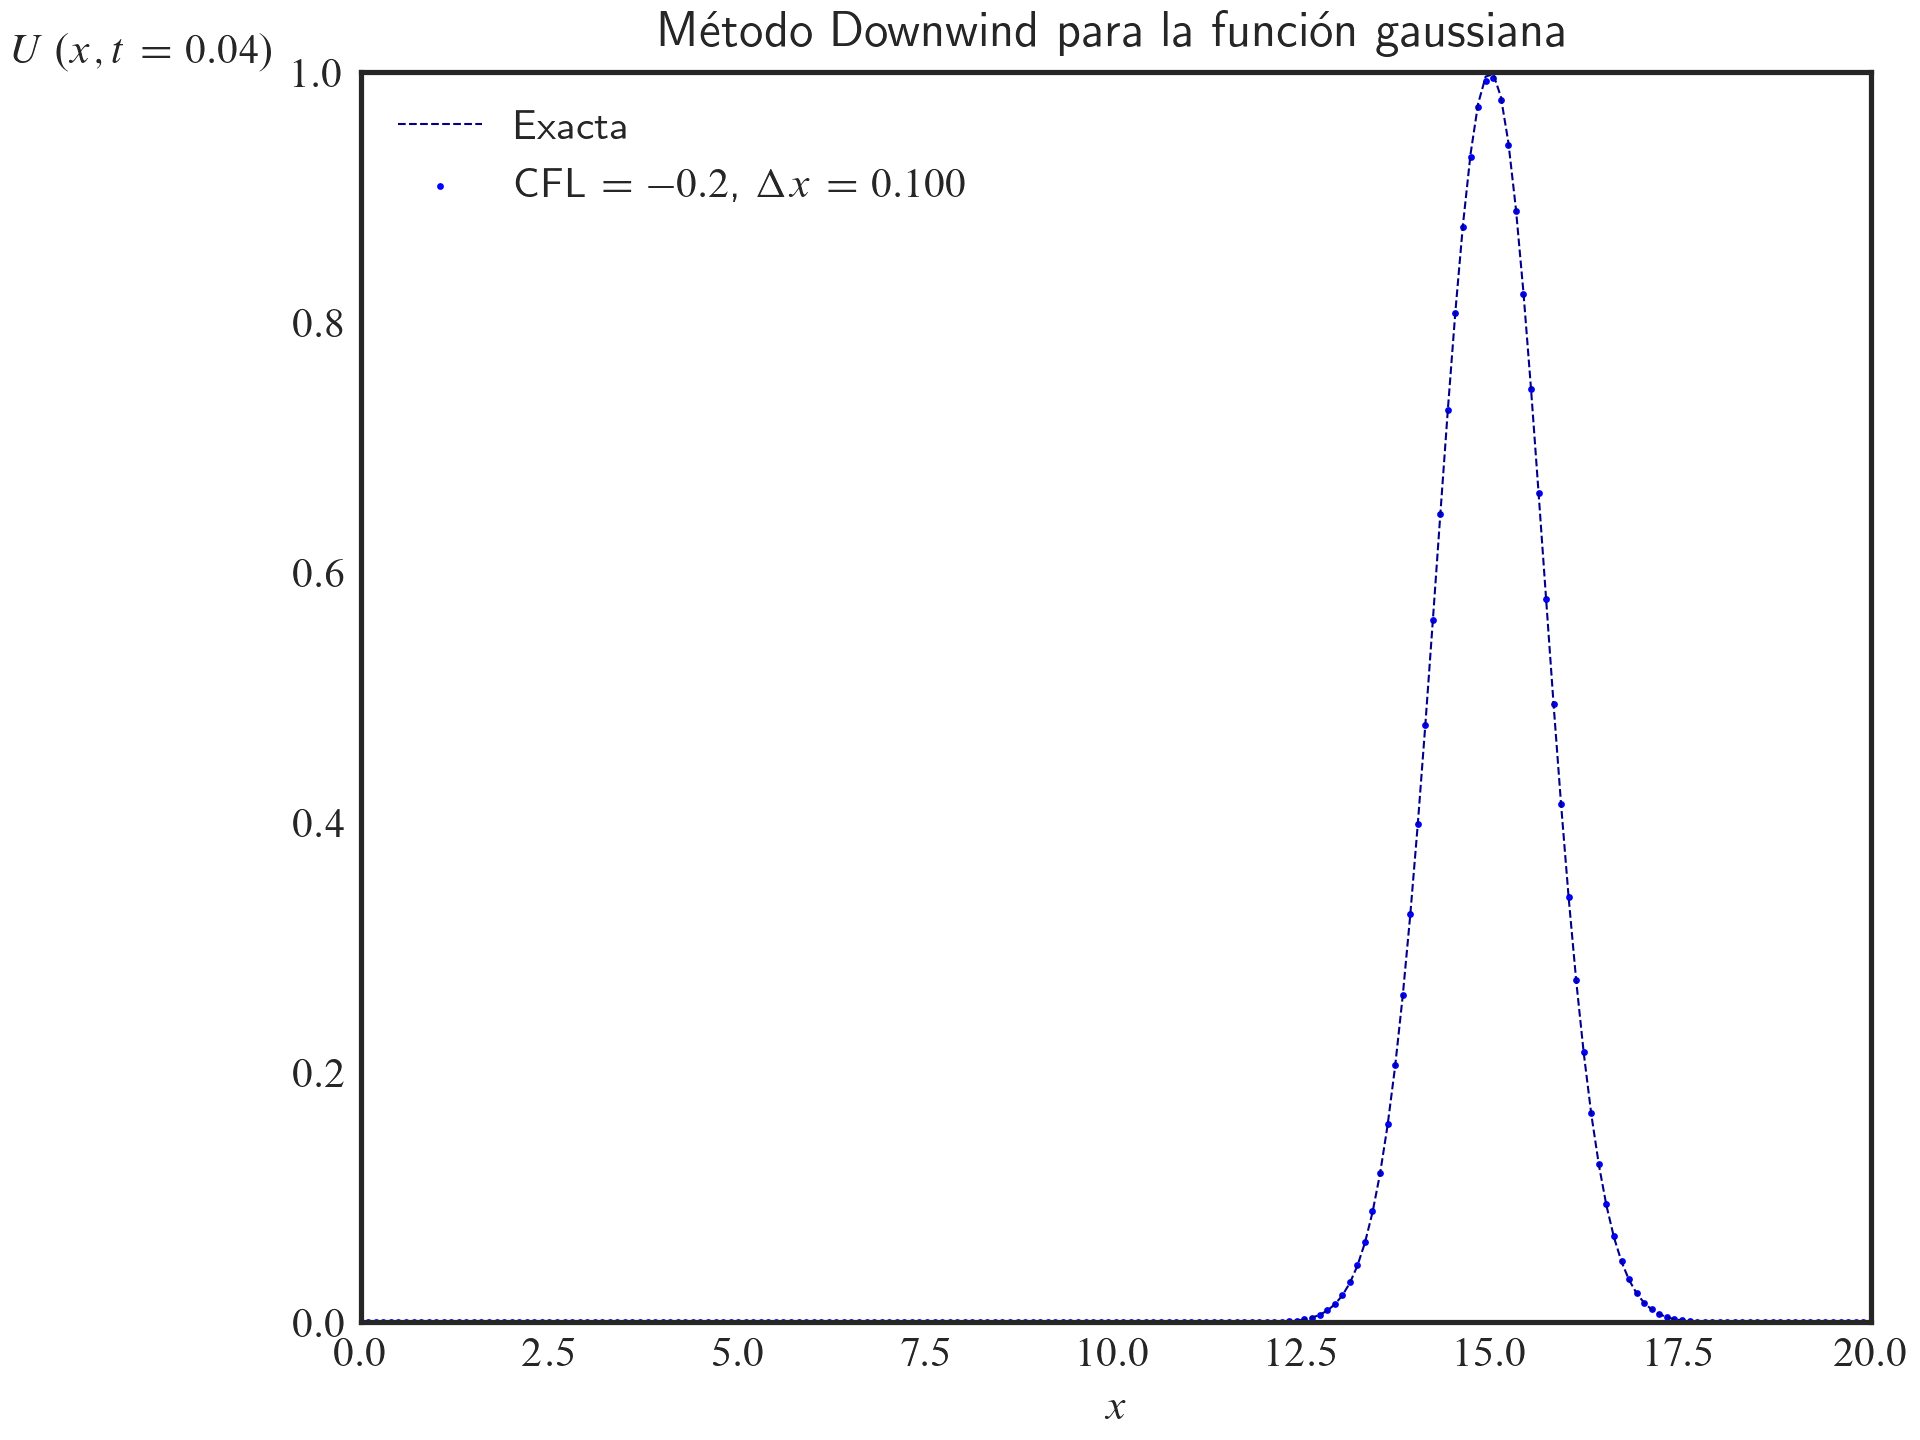
\includegraphics[width=.35\paperwidth]{../snapshots/downwindgaussian1d-2.png}
    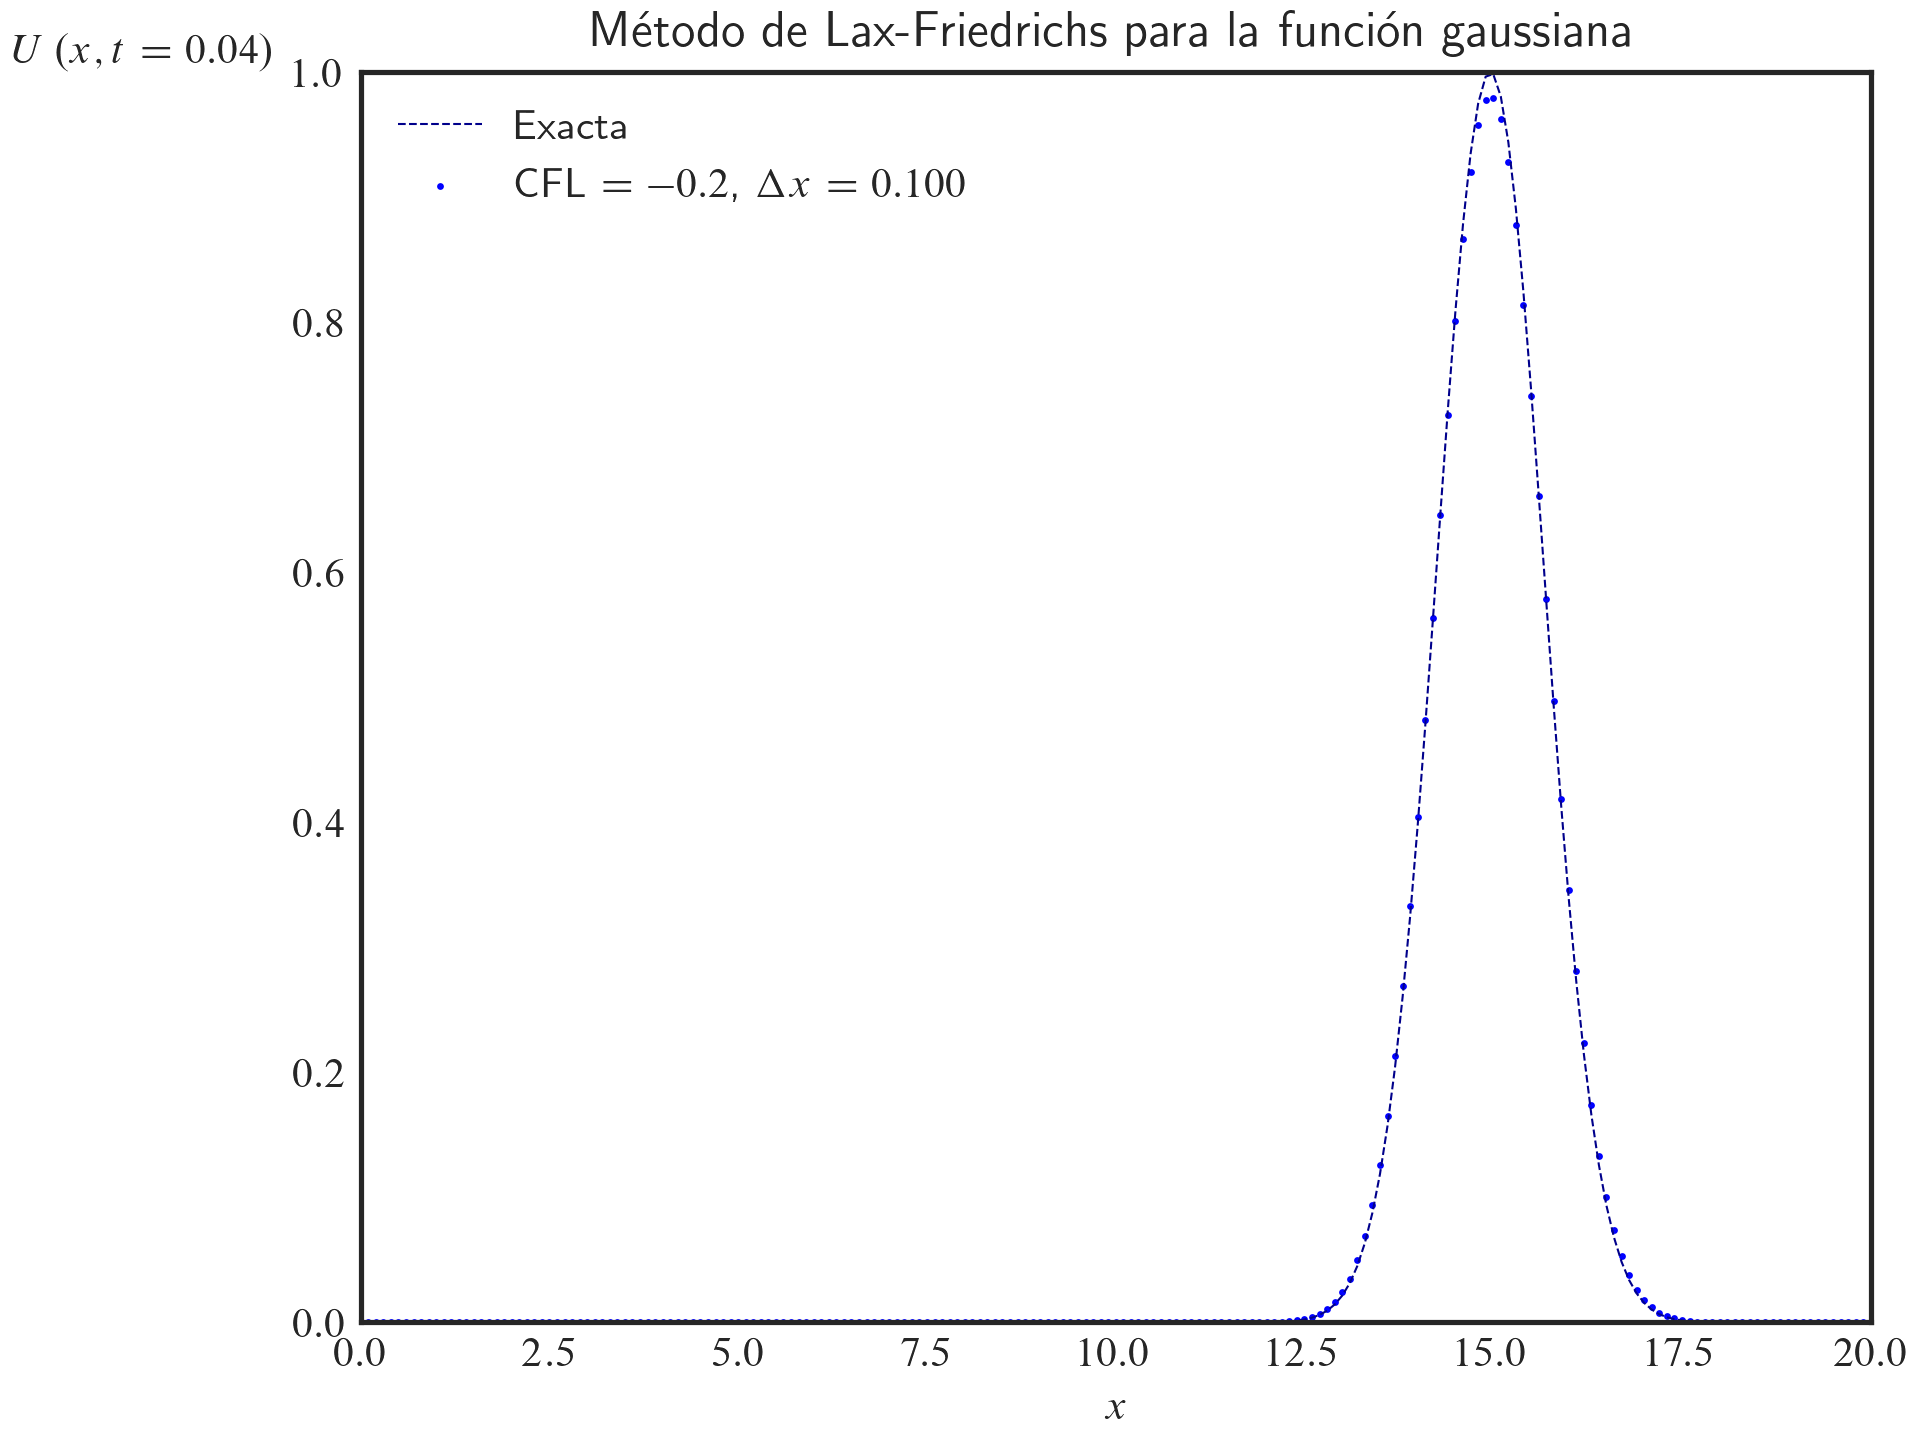
\includegraphics[width=.35\paperwidth]{../snapshots/lax-friedrichsgaussiana1d-2.png}
    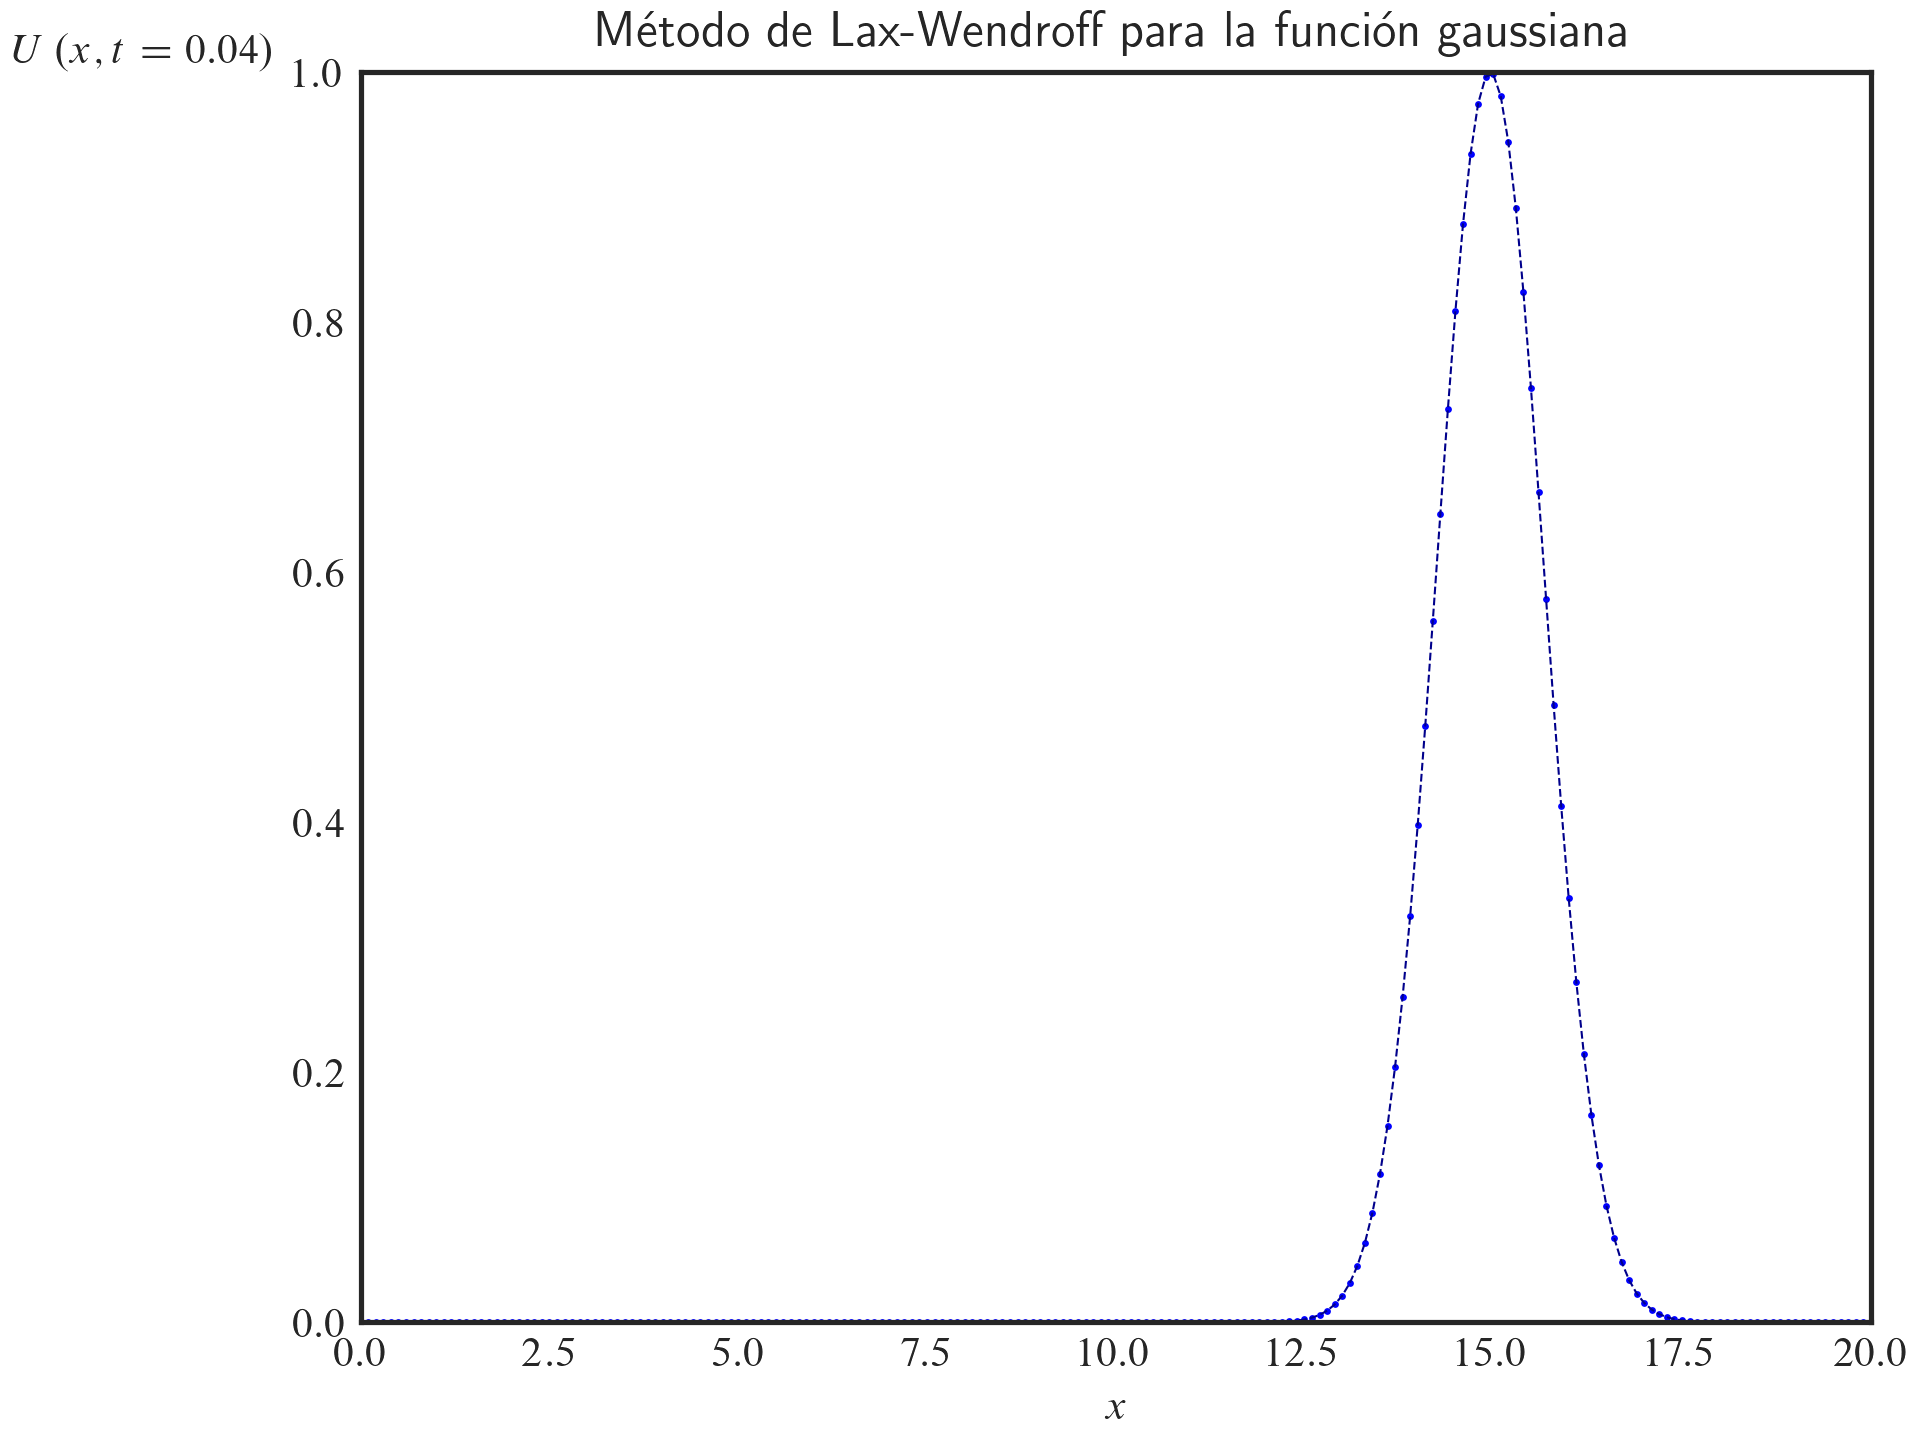
\includegraphics[width=.35\paperwidth]{../snapshots/lax-wendroffgaussiana1d-2.png}
    \caption{Simulación numérica en el tiempo $t_{2}=2\Delta t$.}
    \label{fig:example1t2}
\end{figure}

Observamos cómo, efectivamente, los resultados teóricos concuerdan
con las simulaciones numéricas como era de esperar.
En el capítulo anterior, vimos que el método descentrado downwind y
el de Lax-Friedrichs, ambos, tienen orden de convergencia uno, en
cambio, el método de Lax-Wendroff tiene orden de convergencia dos.
Por lo tanto, como se puede apreciar en las figuras 5.2 y 5.3
(donde se reproduce el mismo experimento pero en los instantes de
tiempo $t_{2}=0.04$ y $t_{40}=0.8$), el método de Lax-Wendroff es el
que proporciona una mejor aproximación de la solución de la ecuación
(5.1) a medida que el tiempo evoluciona.
Por otra parte, también es destacable resaltar el adelanto que
presenta la solución numérica del método de Lax-Friedrichs respecto a
la solución exacta en el instante de tiempo $t_{40}=0.8$.

\begin{figure}[ht!]
    \centering
    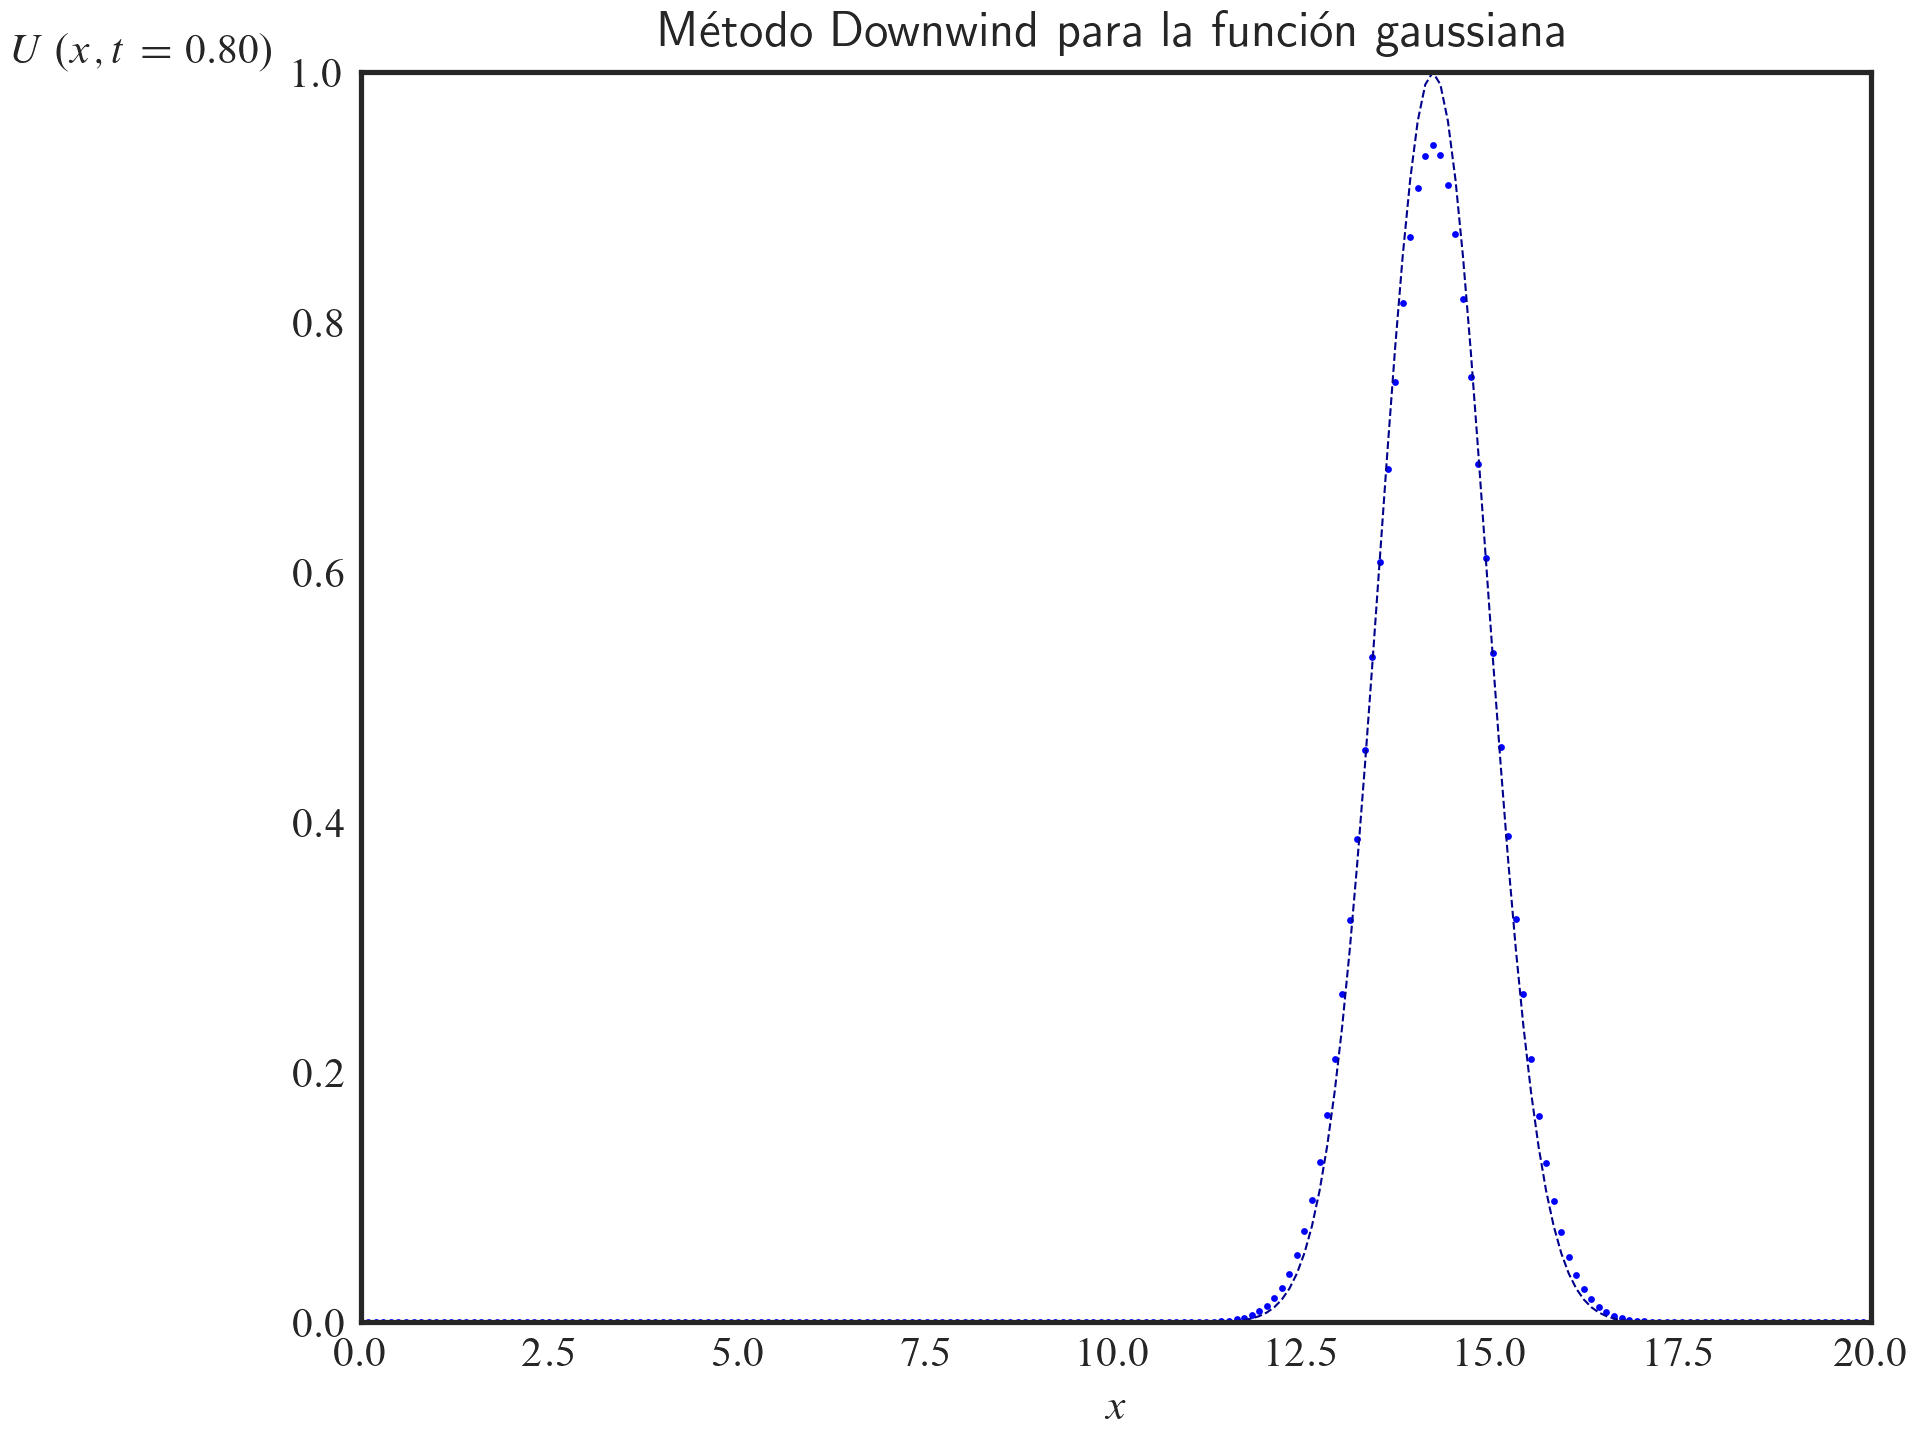
\includegraphics[width=.35\paperwidth]{../snapshots/downwindgaussian1d-40.png}
    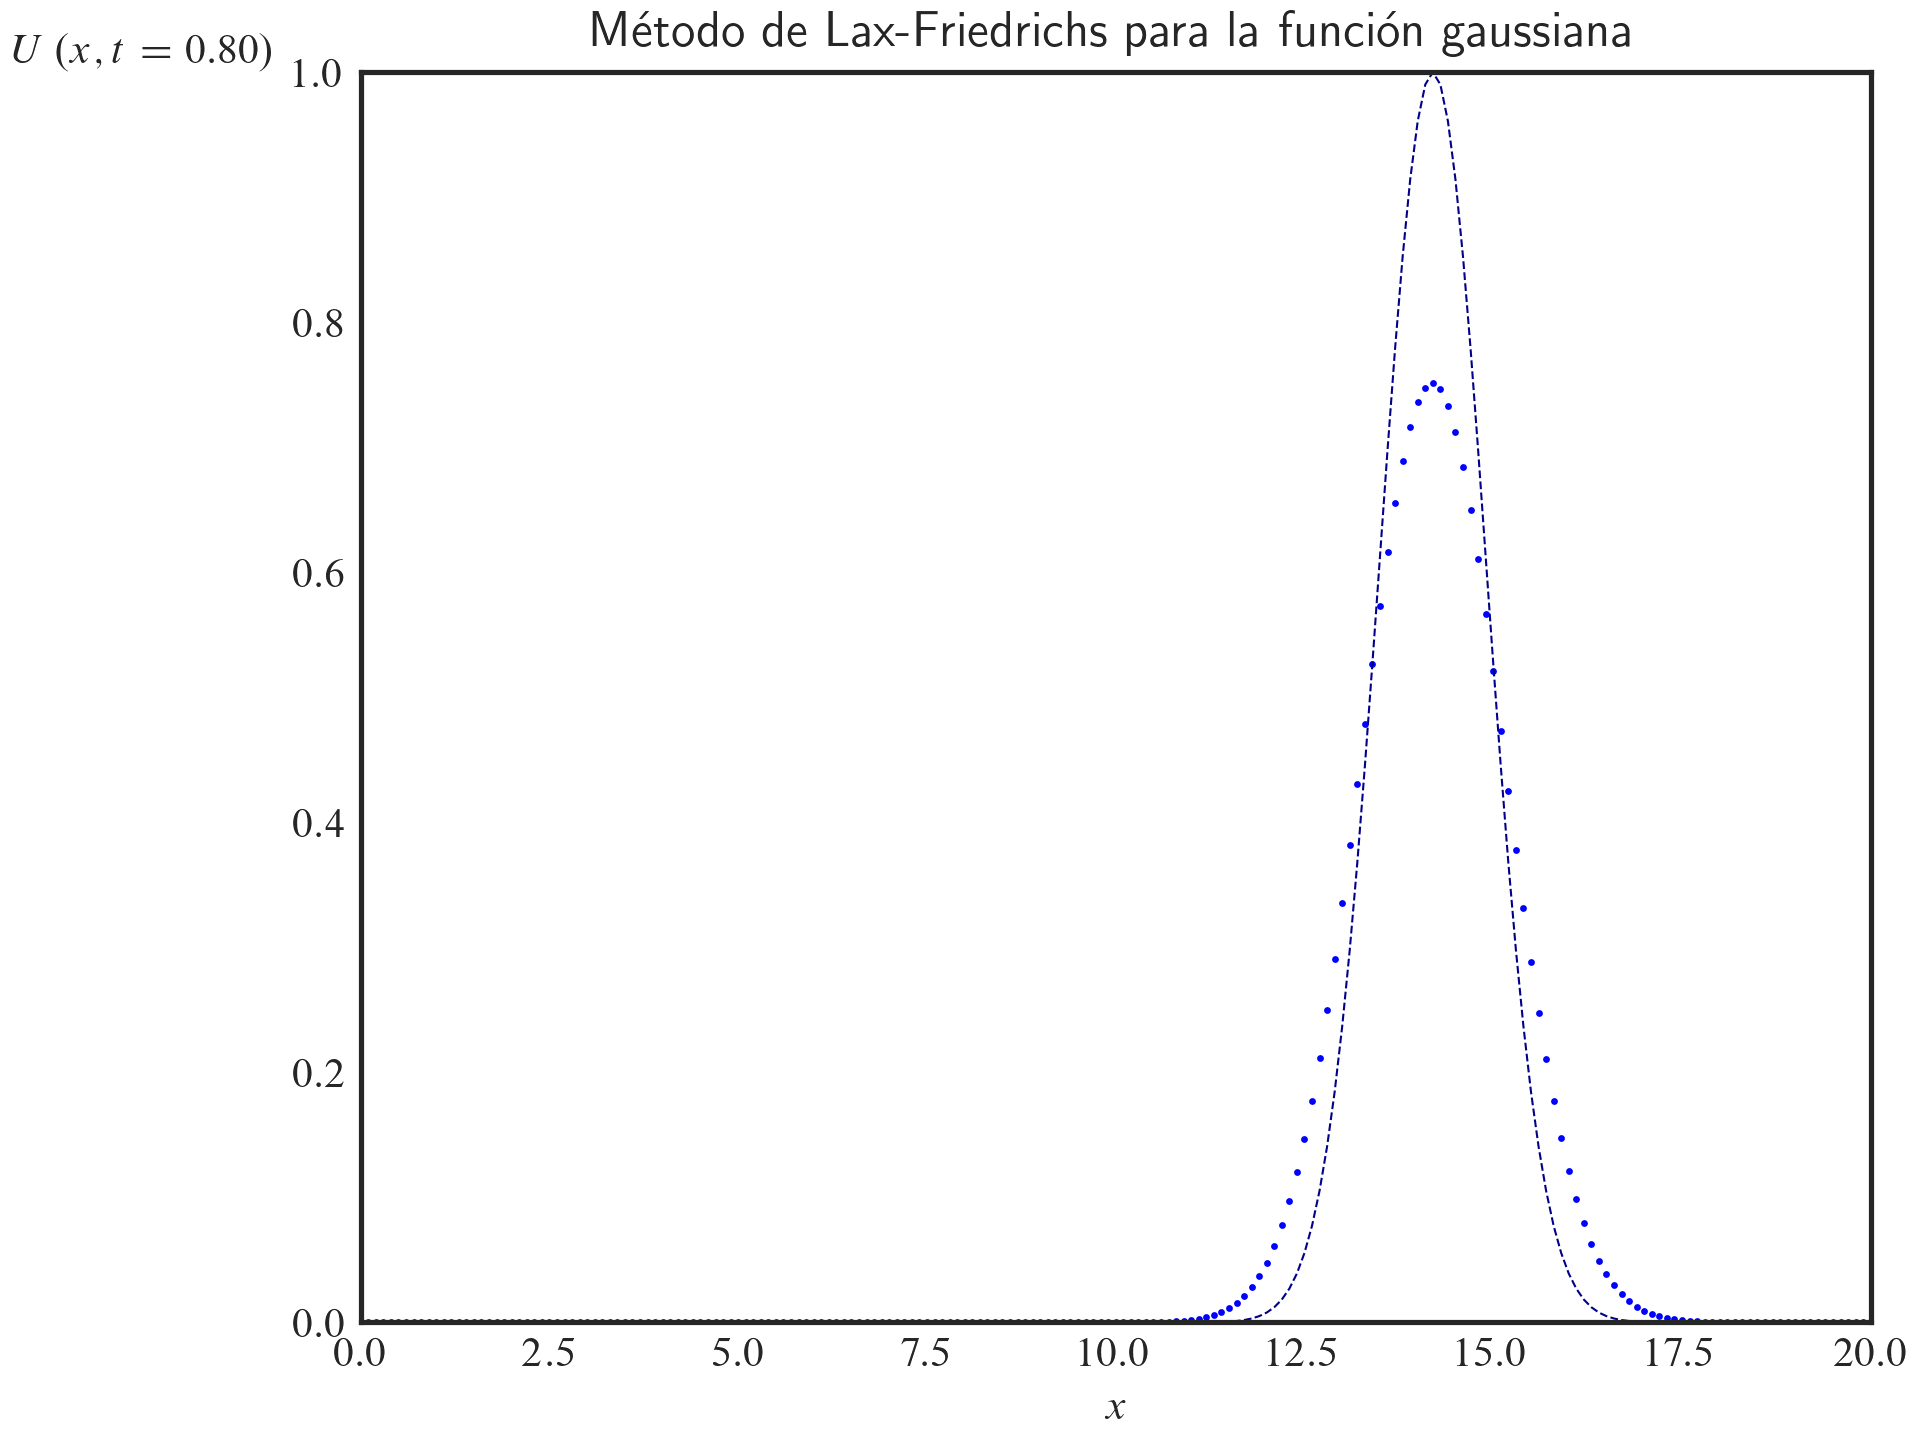
\includegraphics[width=.35\paperwidth]{../snapshots/lax-friedrichsgaussiana1d-40.png}
    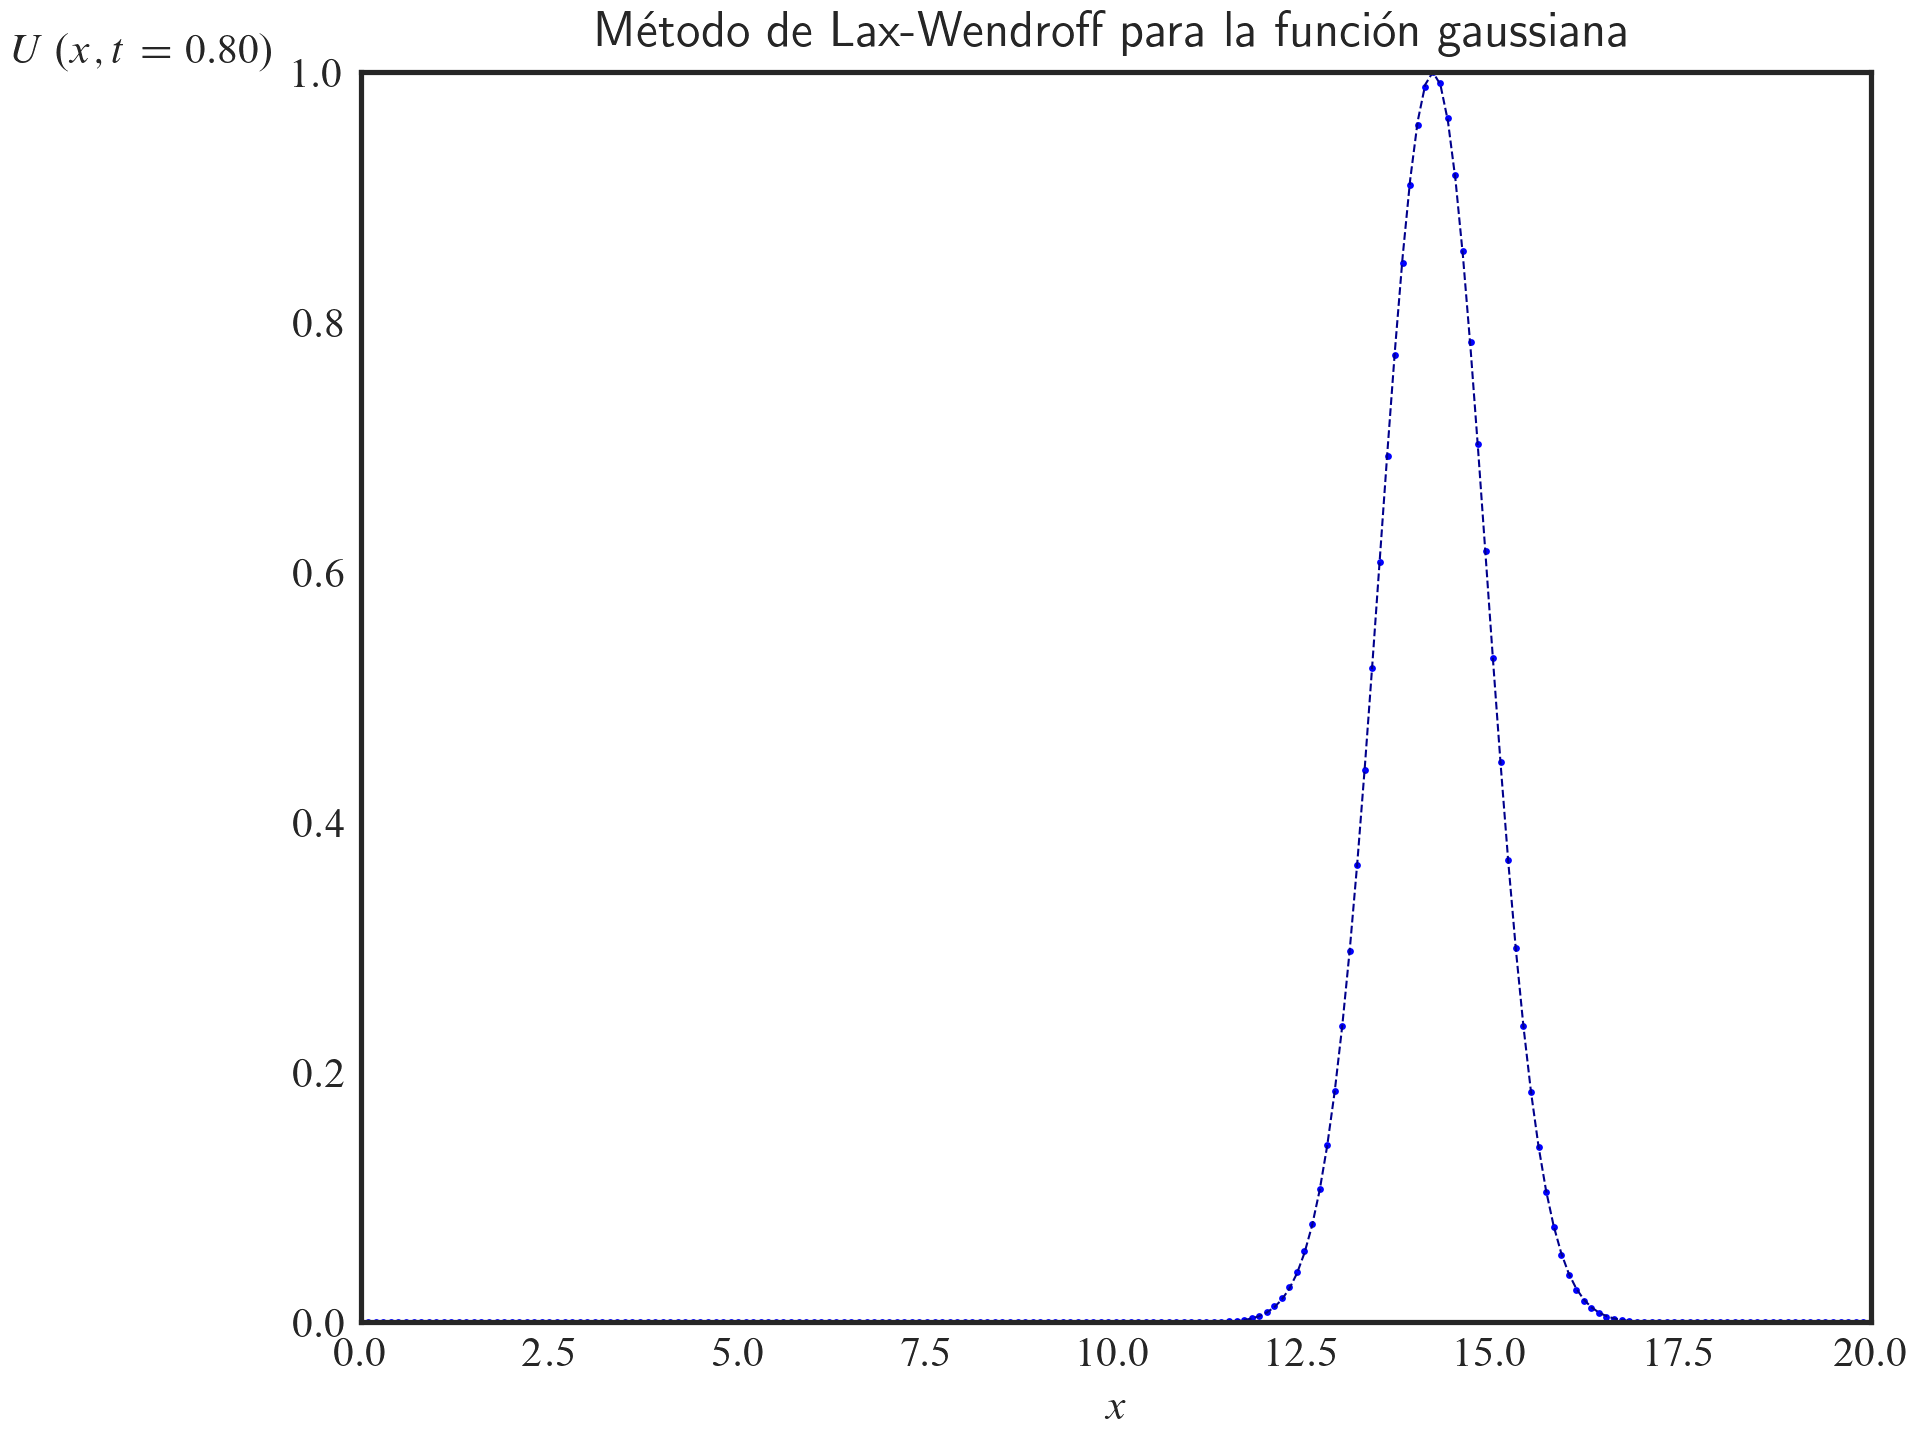
\includegraphics[width=.35\paperwidth]{../snapshots/lax-wendroffgaussiana1d-40.png}
    \caption{Simulación numérica en el tiempo $t_{40}=40\Delta t$.}
    \label{fig:example1t2}
\end{figure}

\subsection*{Ejemplo $2$}

En este ejemplo consideramos el dominio espacial
$\Omega=\left[0,30\right]$, el paso en espacio $\Delta x=0.12$, el
paso en tiempo $\Delta t=0.02$, la velocidad de propagación positiva
$c=1$ (para los que se verifica la condición CFL) y la condición
inicial dada por la función discontinua

\begin{equation*}
    u_{0}\left(x\right)=
    \begin{cases}
        2, & \text{si }x<15, \\
        1, & \text{si }x>15.
    \end{cases}
\end{equation*}

Para este dato inicial calculamos las soluciones numéricas de la
ecuación de transporte (5.1), aplicando el método descentrado upwind,
el método de Lax-Friedrichs y por último, el método de Lax-Wendroff.
Al igual que en el ejemplo anterior, hemos empleado el lenguaje de
programación Python.
Entonces, obtenemos los resultados de las figuras 5.4 y 5.5 (donde se
reproduce el mismo experimento pero en los instantes de tiempo
$t_{2}=0.04$ y $t_{10}=0.2$), para cada uno de los métodos nombrados
junto con la solución exacta y para cada instante de tiempo
considerado.

\begin{figure}[ht!]
    \centering
    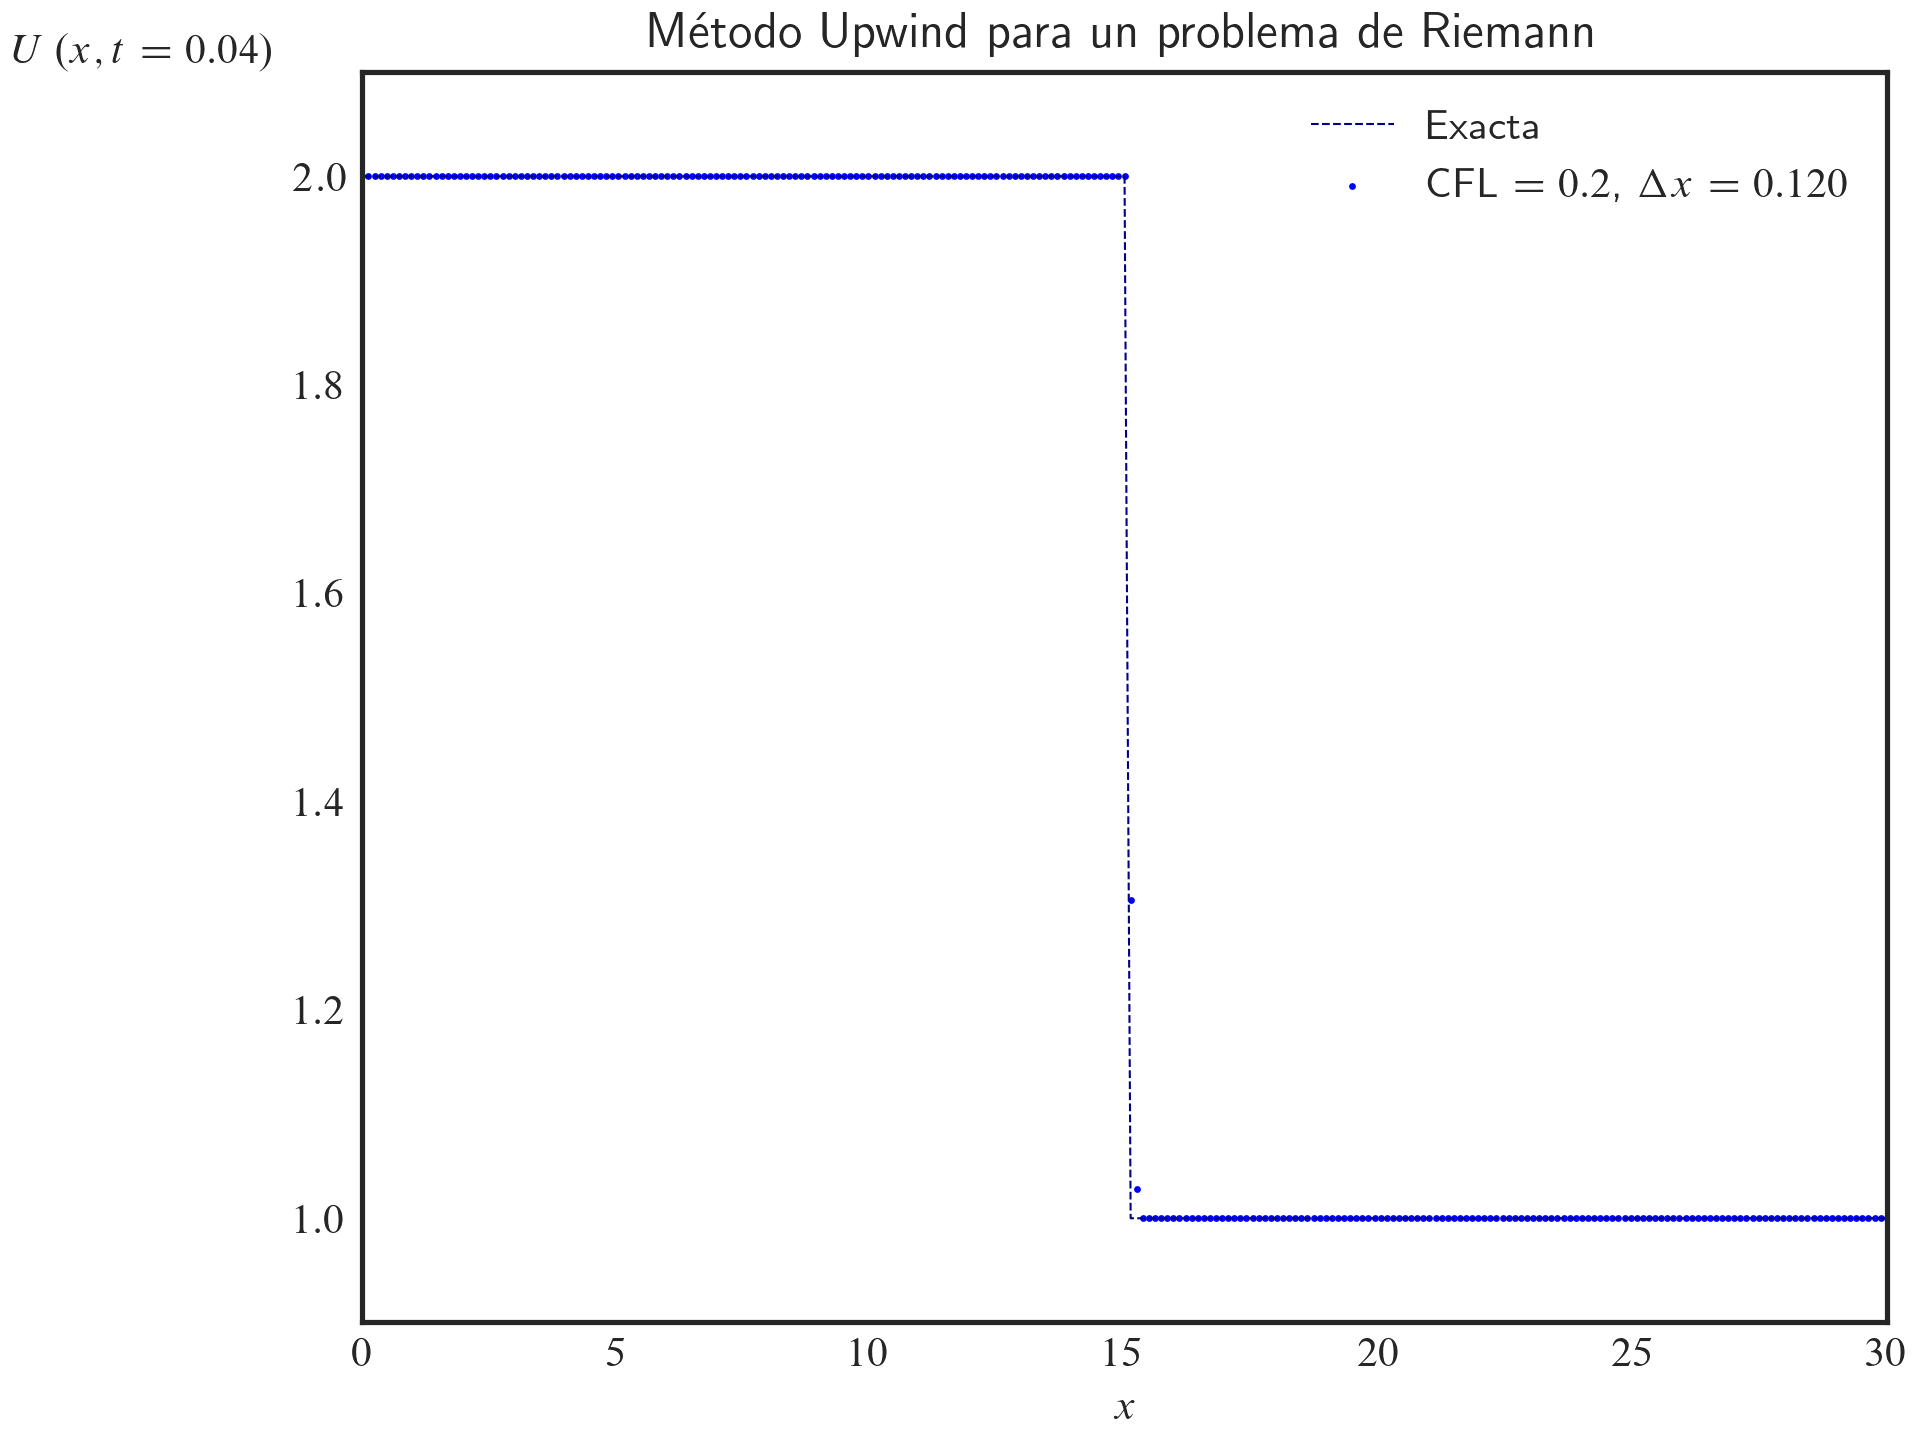
\includegraphics[width=.3\paperwidth]{../snapshots/upwindheaviside1d-2.png}
    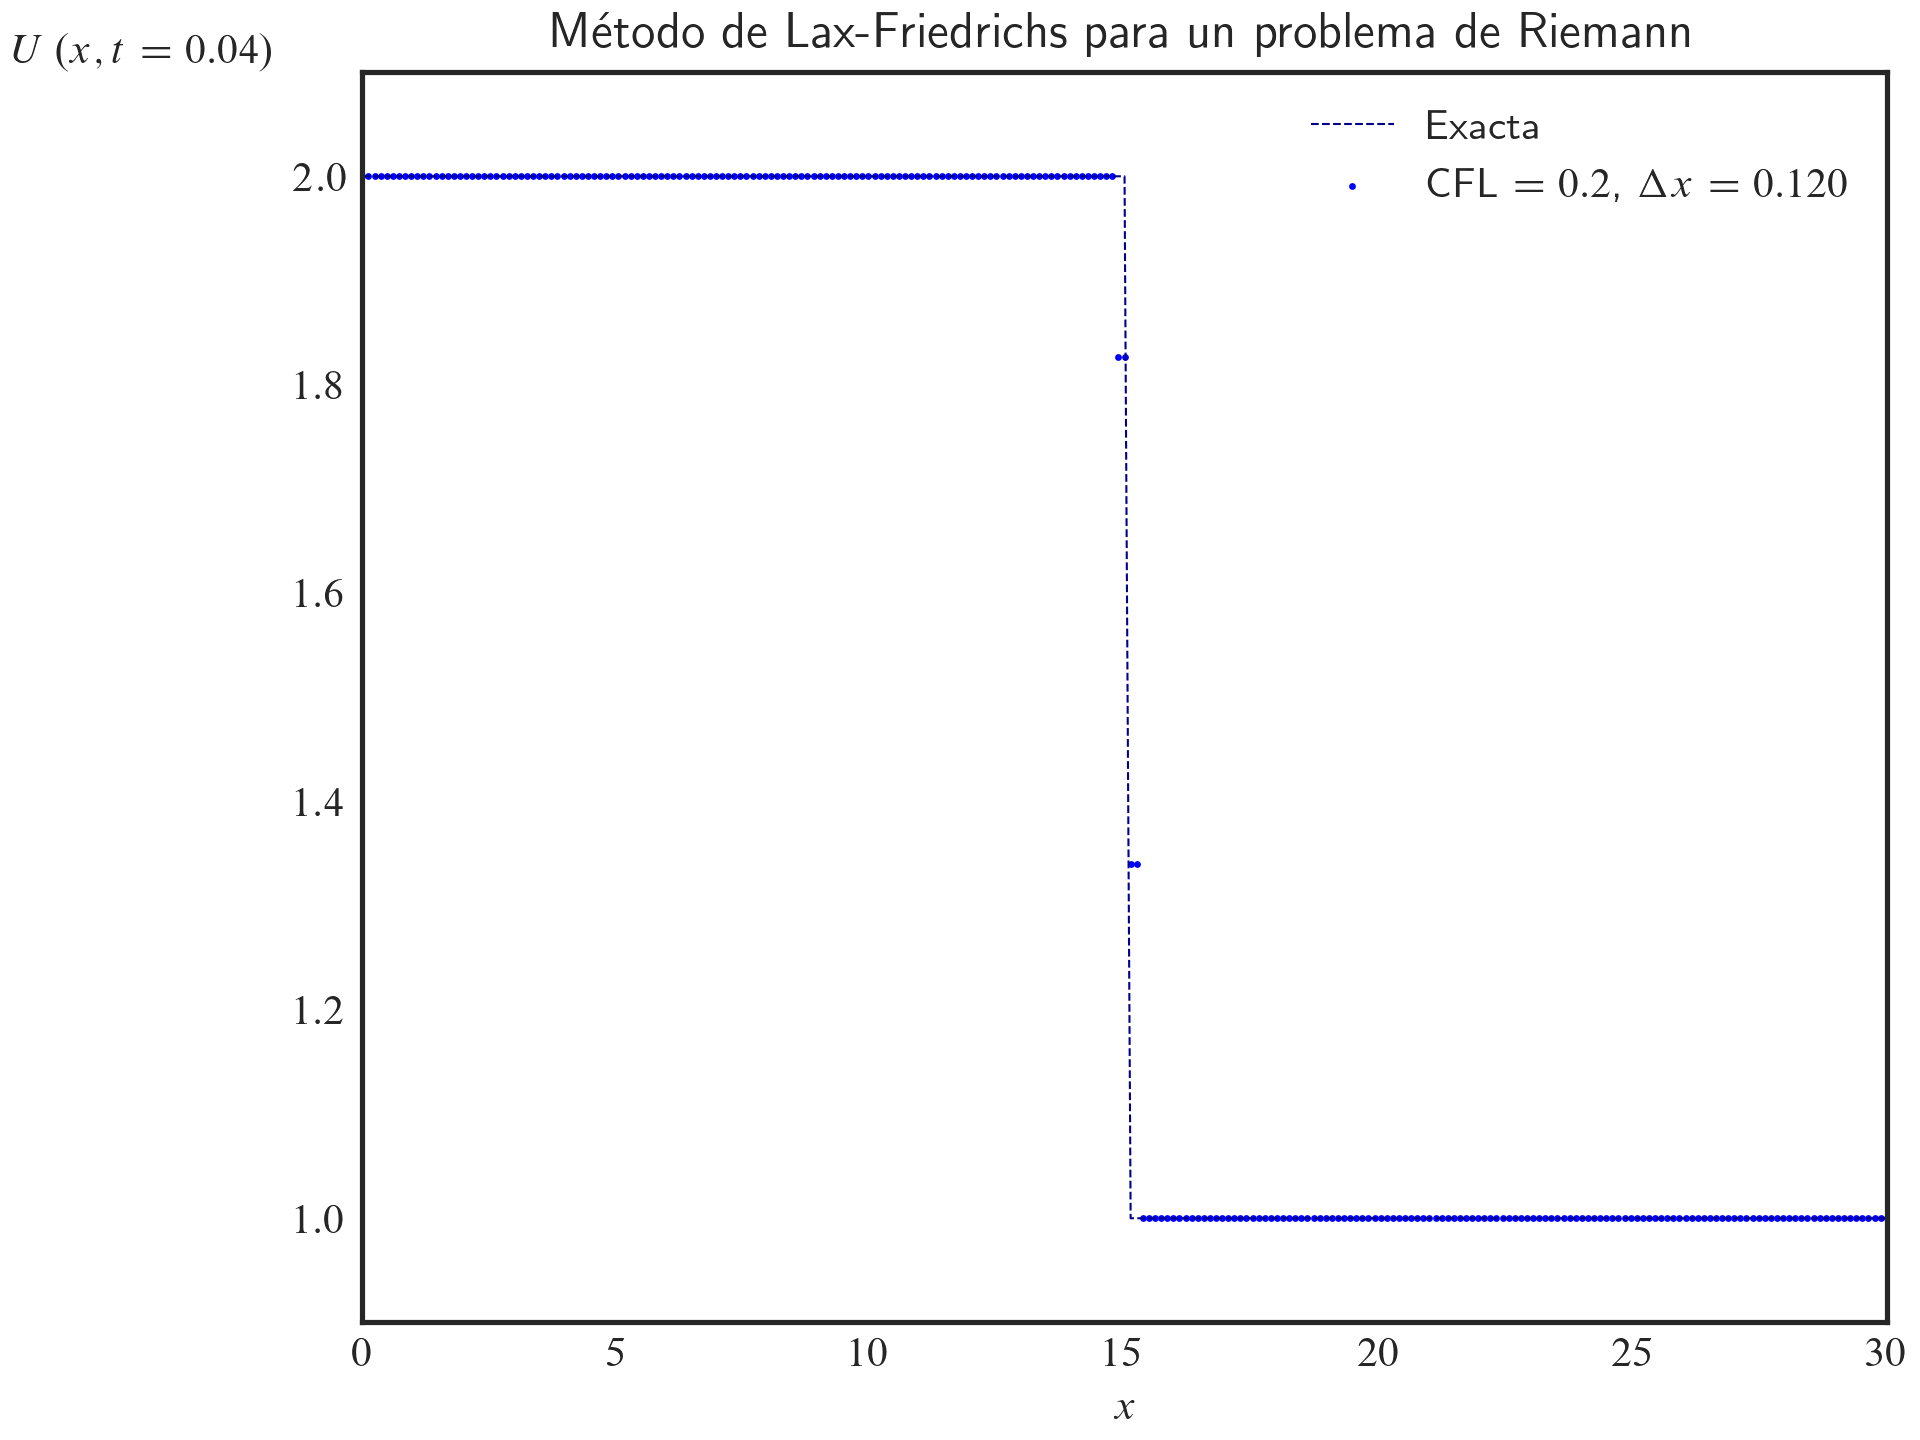
\includegraphics[width=.3\paperwidth]{../snapshots/lax-friedrichsheaviside1d-2.png}
    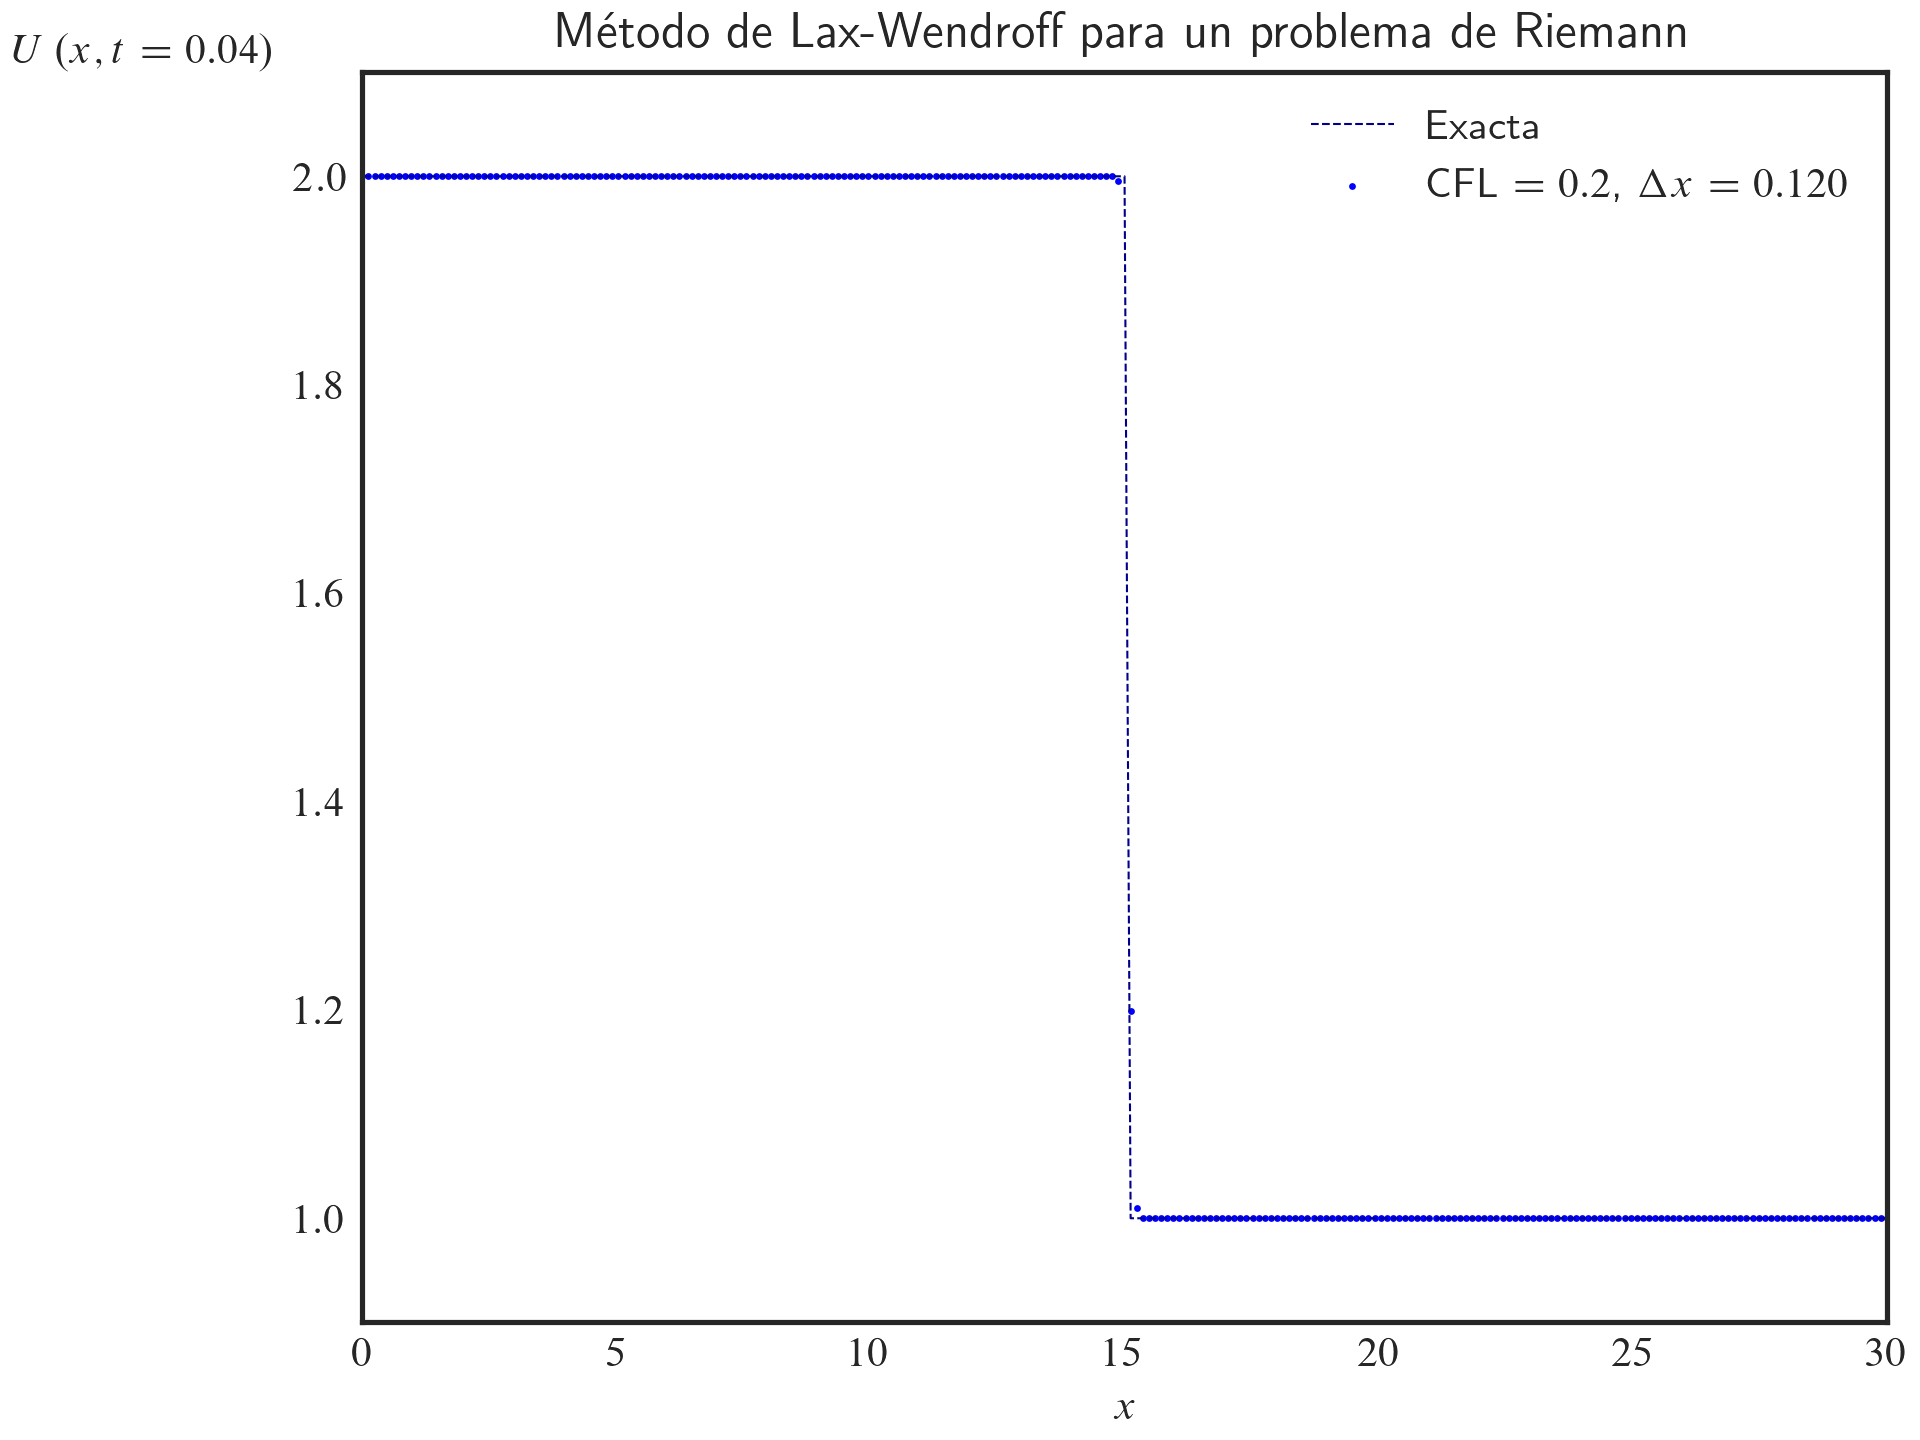
\includegraphics[width=.3\paperwidth]{../snapshots/lax-wendroffheaviside1d-2.png}
    \caption{Simulación numérica en el tiempo $t_{2}=2\Delta t$.}
    \label{fig:example1t2}
\end{figure}

En la figura 5.5 (experimento en el instante de tiempo $t_10=0.2$),
se puede apreciar que el método aguas arriba aproxima bien la
solución pero contiene una pequeña disipación numérica entorno a la
discontinuidad, en donde disminuye la precisión.
Aunque mayor es la disipación numérica que provoca el método de
Lax-Friedrichs en dicha discontinuidad.
Por otra parte, es destacable resaltar el hecho de que el método de
Lax-Wendroff provoque las denominadas oscilaciones espurias en las
regiones próximas a la discontinuidad.
Este hecho es bien conocido y está documentado en [12].
Sin embargo, es más preciso en aquellos puntos donde la solución es
más regular.

\begin{figure}[ht!]
    \centering
    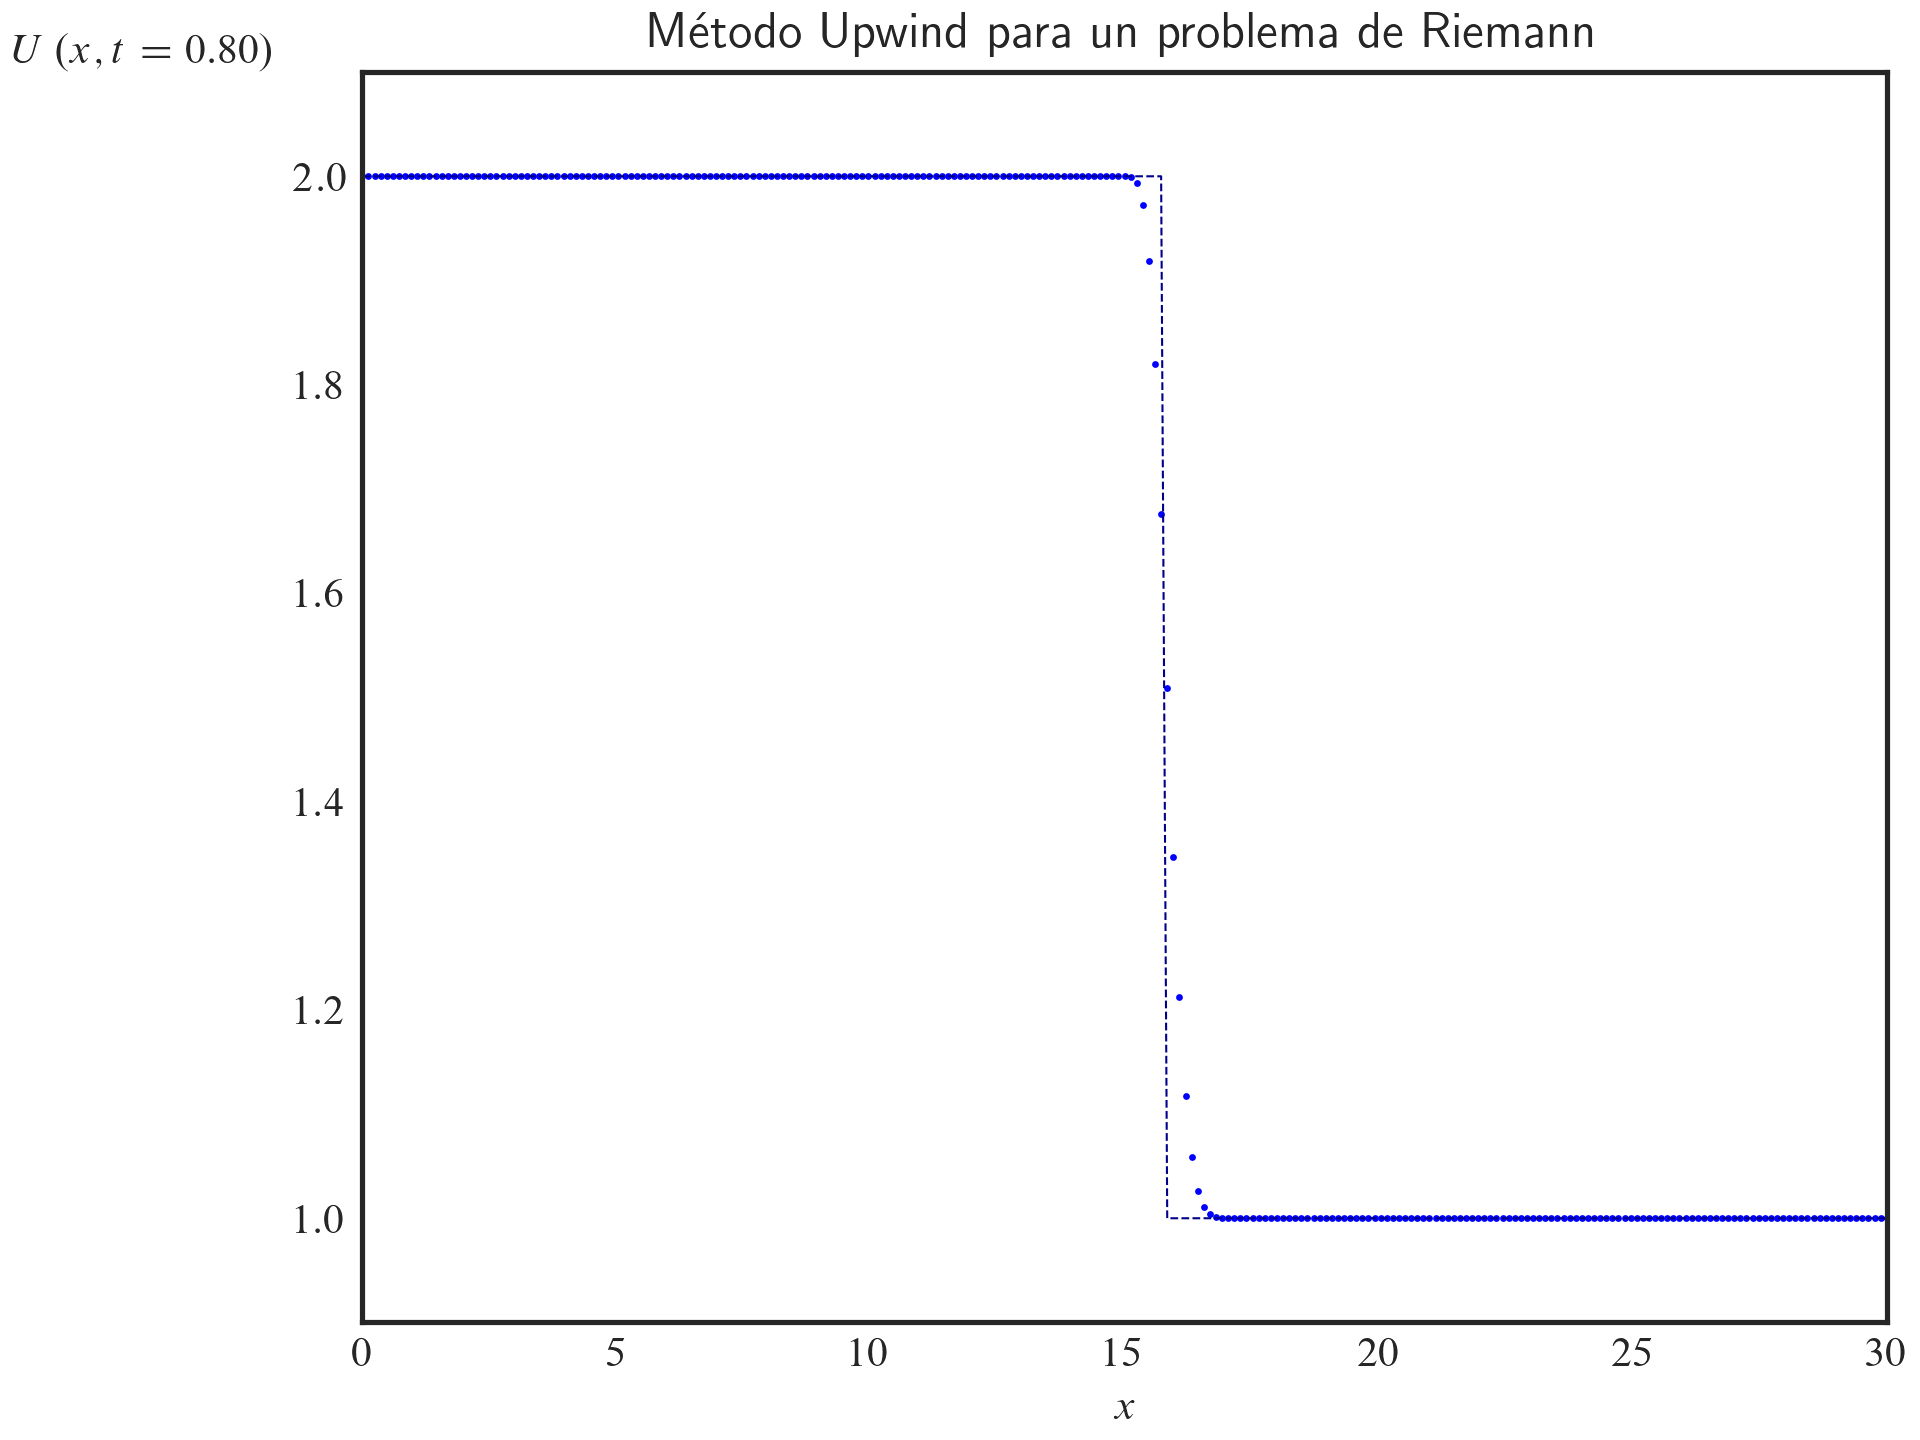
\includegraphics[width=.3\paperwidth]{../snapshots/upwindheaviside1d-40.png}
    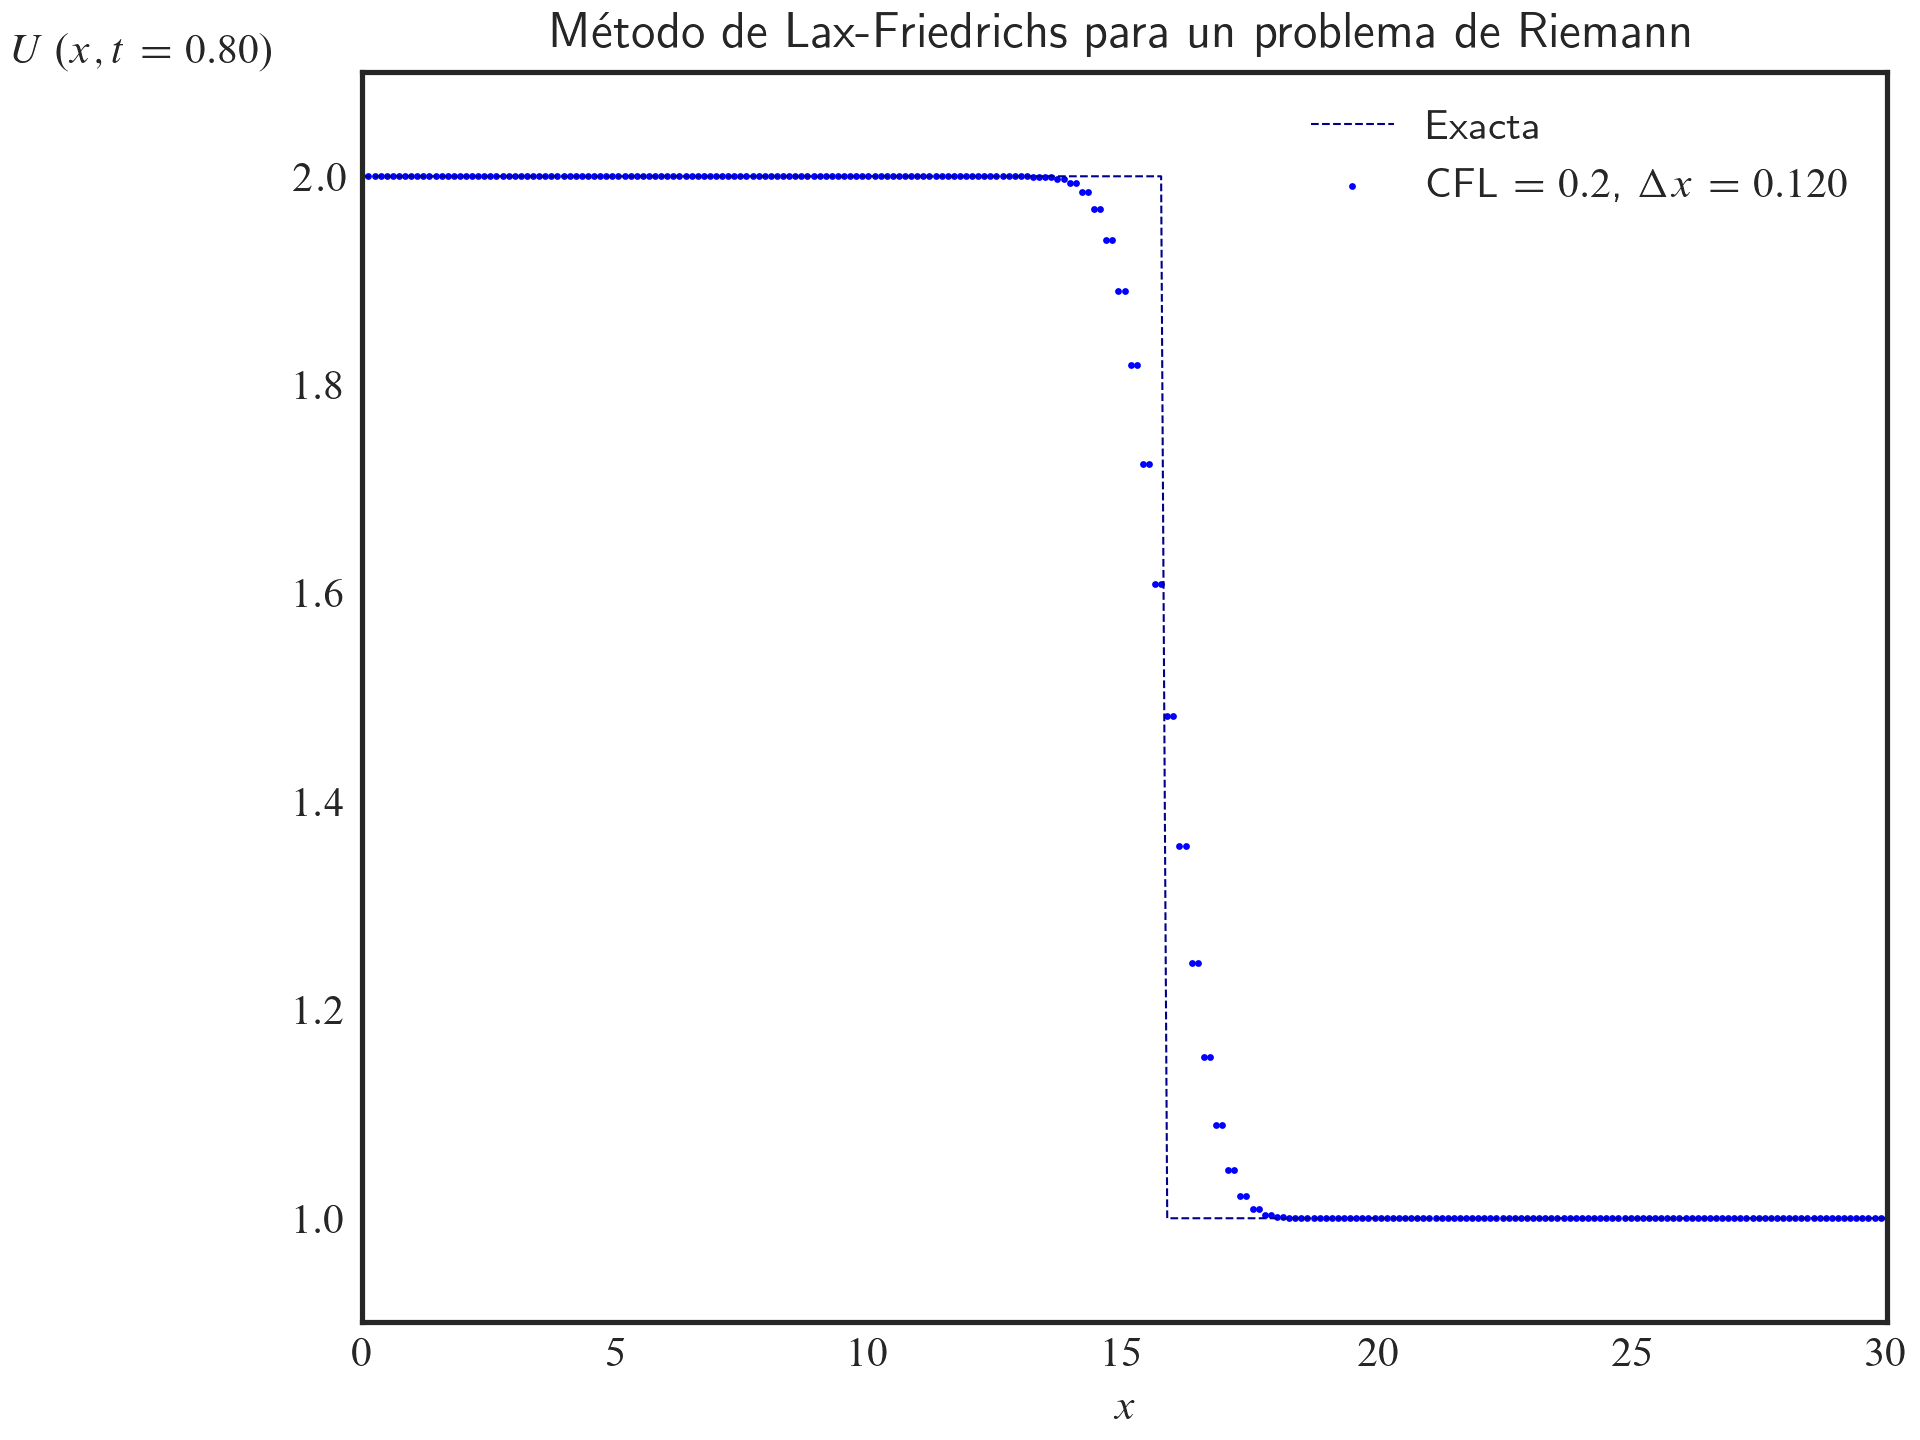
\includegraphics[width=.3\paperwidth]{../snapshots/lax-friedrichsheaviside1d-40.png}
    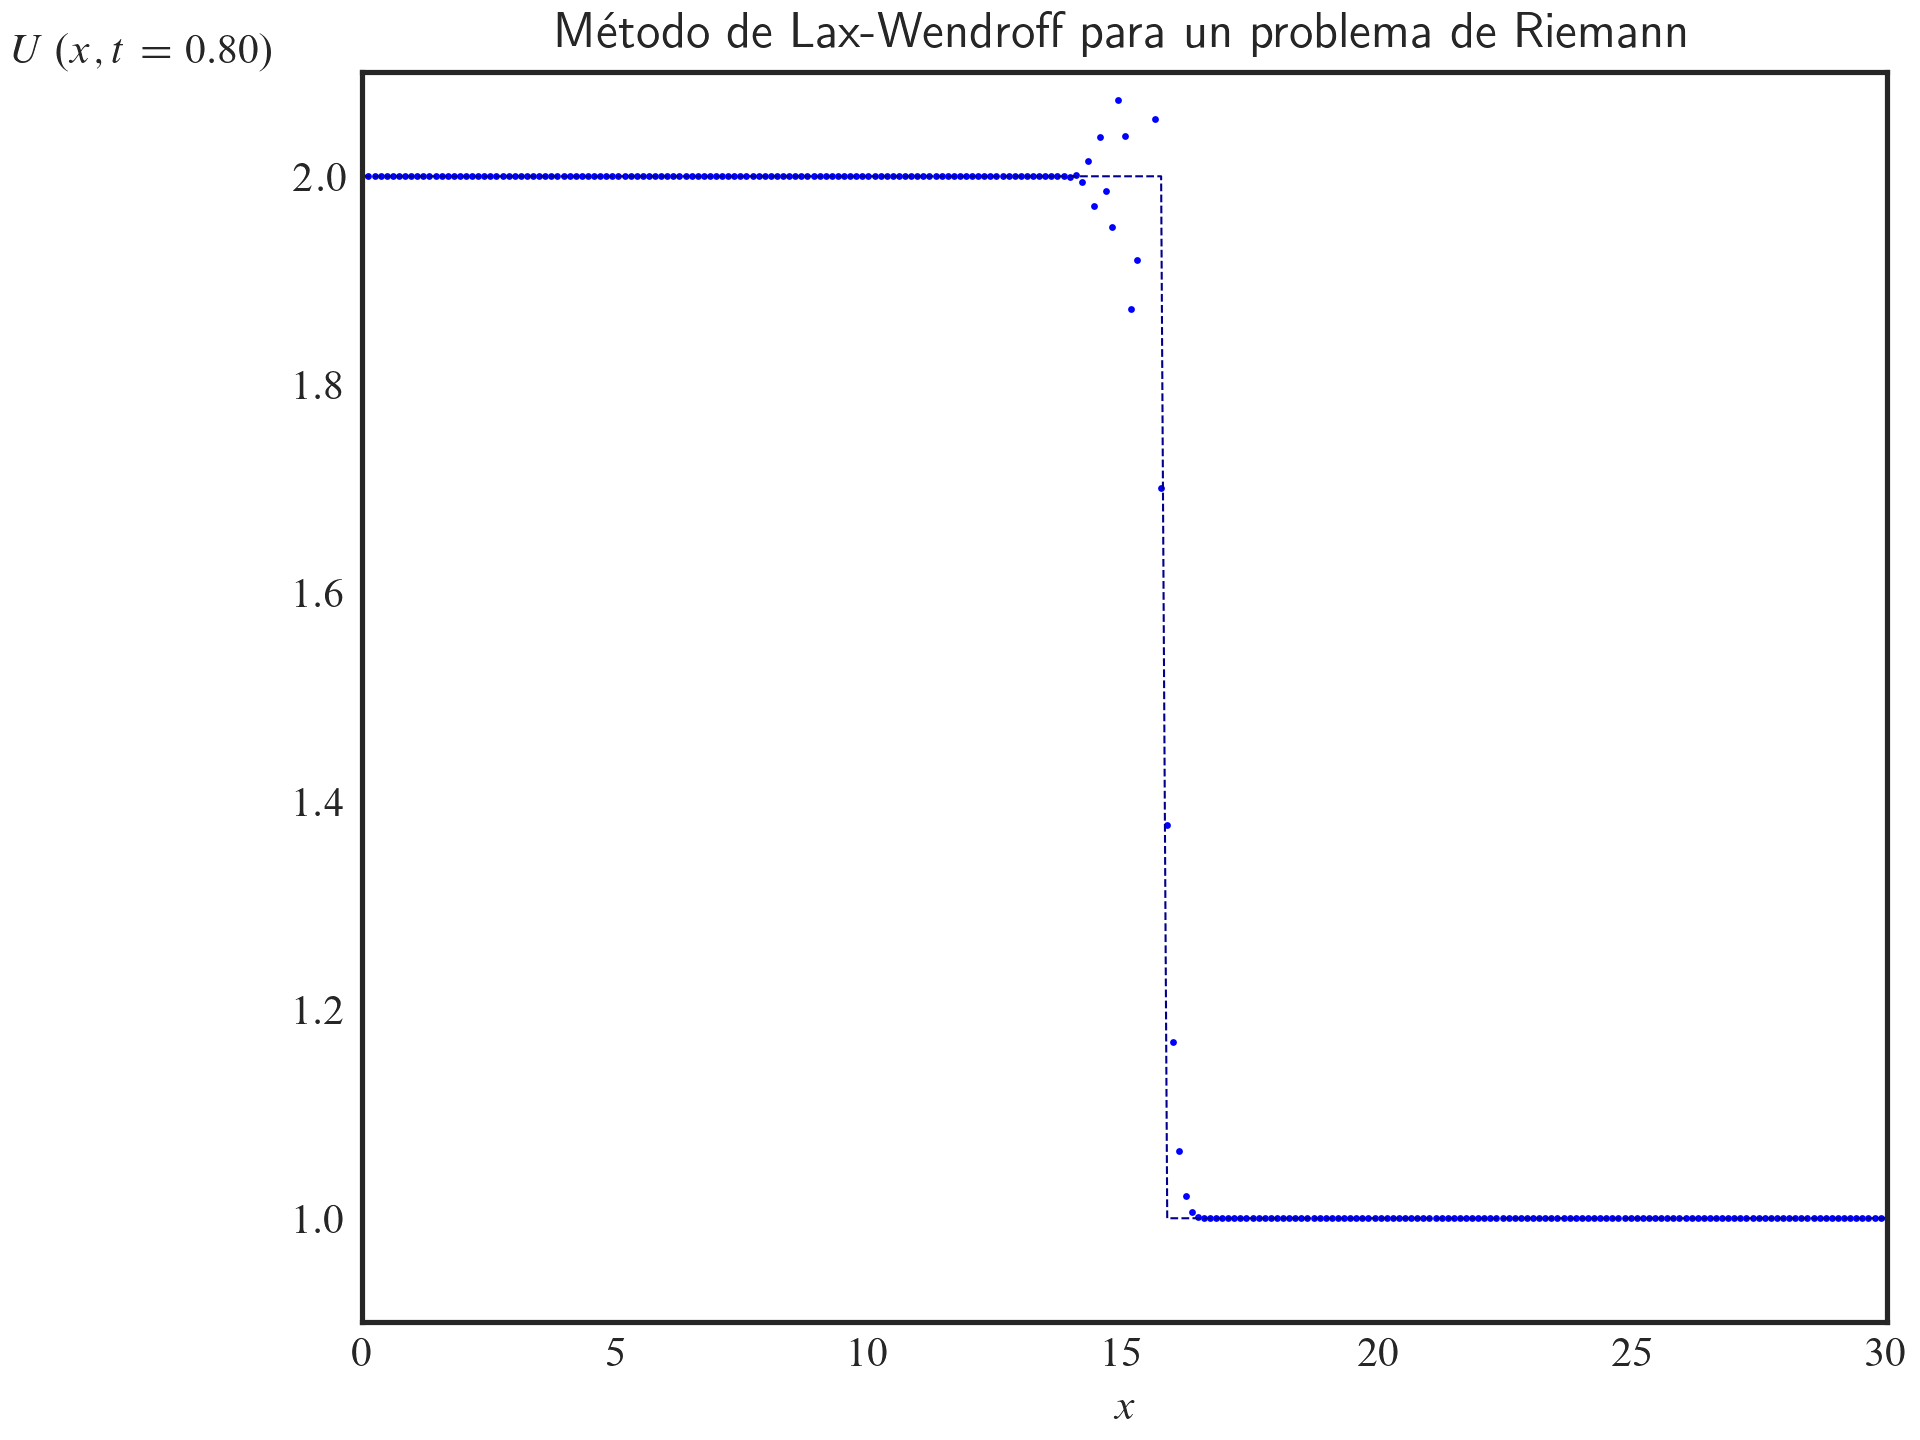
\includegraphics[width=.3\paperwidth]{../snapshots/lax-wendroffheaviside1d-40.png}
    \caption{Simulación numérica en el tiempo $t_{40}=40\Delta t$.}
    \label{fig:example1t2}
\end{figure}